\chapter{Cooperative Motion Planning and Decision-Making for MVS: Architecture Overview} \label{sec: CooperativeNavigation_GlobalOverview} \label{chap:chapter2}




\begin{abstract}
This chapter is devoted to providing a comprehensive overview of MVS control architecture. It delves into an exploration of pertinent literature, examining the various applications of MVS across different domains. The chapter sheds light on the paradigms employed in constructing MVS control architecture. Furthermore, it offers a detailed literature review of MVS applications within complex and dynamic environments.
    
\end{abstract}


\textbf{Contents}
\vspace{0.15cm}
\hline
\hspace{2cm}
\localtableofcontents
\hspace{2cm}
\hline











\section{Introduction}
% TODO
%% Give an introduction about the importance of AV in acadimia and link it to Zhing's diagram
%% Introduce the idea of acadimia being interessted about the MVS and give one old reference about MVS to prove that MVS are pretty old a topîc of interest in acadimia 
%% donner un cahier des charges de sur quoi le MVS doit respecter un peu comme le fait Zhang (page 39)
%% Need to introduce the idea of several types of architecture (centralized/ distributed/ hybride) 
%%  ajouter une section sur les architecture multi-controller/ behaviors pour introduire le fait que j'ai plusieurs behaviors (voir livre lounis page 17 et la thèse de Vilca surement) 
%% Need to introduce the idea that we do have a variaty of methods that rely on several levels (decision, communication, control) to precise our scoop which is (decision and control) not communication. 


In the recent years, the automotive research and industry has undergone a profound transformation, driven by rapid advancements in technology and a growing emphasis on safety, sustainability and efficiency. At the forefront of this evolution, one concept is pointed to revolutionize the way we think about transportation: Multi-Vehicle System (MVS). These cutting edge technologies represent the fusion of several years of development of the automated vehicles, connectivity and automotive engineering, promising to reshape not only the way we move and travel but also our urban environment and our roads. 




The primary objective of this chapter is to provide an extensive overview of the MVS control architecture, along with the examination of the relevant literature concerning the utilization of MVS across diverse applications. Section \ref{sec:control_architecture_for_MVS} outlines the various modules and process integrated in the MVS control architecture. In Section \ref{sec:MVS_control_Architecture}, an insight into the paradigms employed in constructing the MVS control architecture is presented. Formation control stands as an important aspect of the MVS paradigm, and thus, in Section \ref{sec: formation_control_theory}, a comprehensive review of various formation control approaches is conducted. Lastly, Section \ref{sec:review_MVS_application} provides a literature review highlighting MVS applications within complex environments.  


% je peux continuer cette section avec l'explication de ce qu'on va trouver dans les sections plus bas à savoir expliquer les architecture, et les méthodes utilisées avec le classement --- un truc en mode in this section .... blablabla 

\section{Control architecture for MVS} \label{sec:control_architecture_for_MVS}
% enfaite deja là on commence a parler de l'architecture du véhicule. 
Automated Vehicles (AVs), known as self-driving cars or autonomous vehicles, have captured the imagination of the public, scientists and industry alike during three decades. These vehicles leverage sophisticated sensors, complex decision-making processes and real-time data analysis to navigate the roads with minimal to absence of human intervention. The promise of improved safety, enhanced energy management, reduced congestion, and increased accessibility has fueled intense research and development. One consensus started to emerge between the contributors to the AVs developments; to take full advantages of the AV technology, AVs must collaborate with the road users.

On the other hand, MVS takes the concept of driving automation to the next level by introducing a collaboration level between vehicles, infrastructures, and even pedestrians. This inter-connectivity has the potential to induce numerous benefits such as enhancing safety, more efficient energy consumption and real-time traffic optimization (cf. Section \ref{sec: CooperativeNavigation-Scenarios Overview}).  

The autonomous management of a fundamental MVS essentially encompasses five core process as depicted in Figure \ref{fig:MVS_architecture_concept}, which are detailed as follows: 

\begin{figure}[!h]
        \centering 
        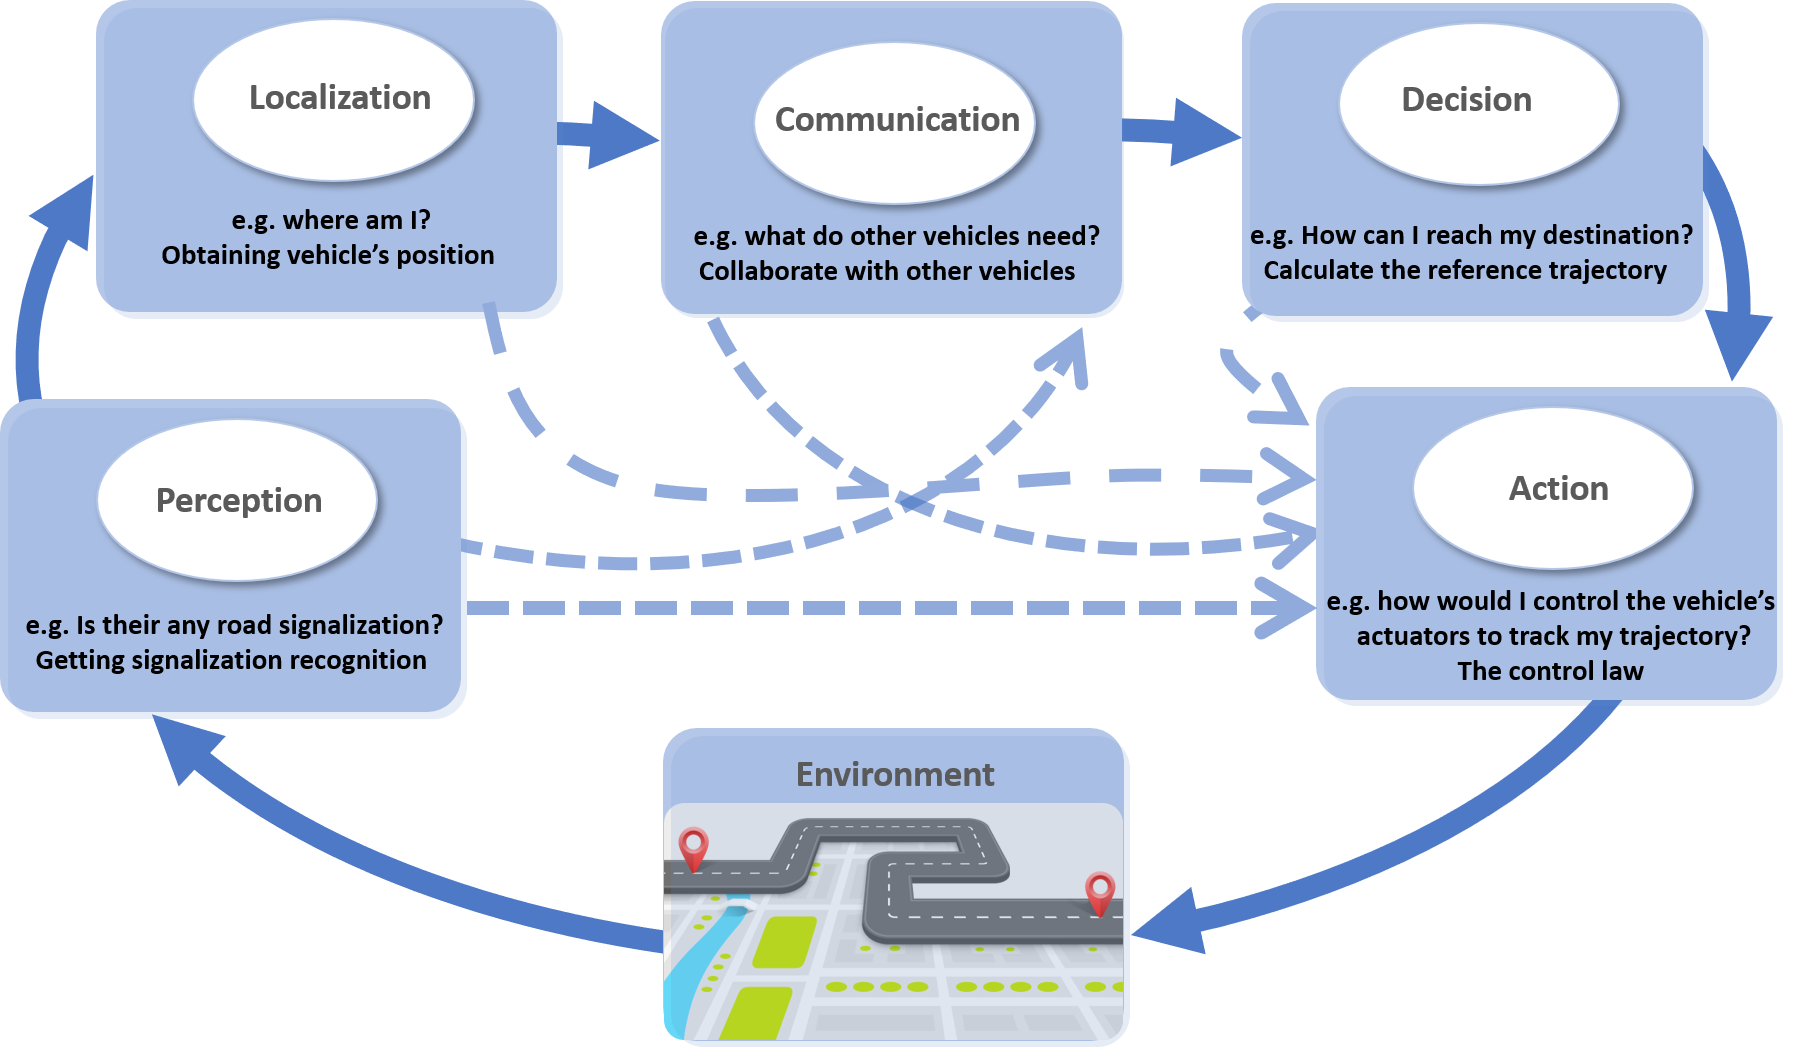
\includegraphics[width=12cm,height=18cm,keepaspectratio]{chapters/Chapitre_3/Figures/Diagram_MVS_architecture.png}
       % \vspace{-2.3mm}
        \caption{Reference control scheme for MVS, adapted from \cite{ventura2015safe}}
        \label{fig:MVS_architecture_concept}
           %     \vspace{-5mm}
        \end{figure}

\subsection{Perception module} \label{sec: perception} 
The perception module plays a pivotal role in gathering precise data for both the vehicles part of the MVS and the surrounding vehicles. It relies on a combination of sensors designed for distinct purposes: 
        \begin{itemize}
         \item Proprioceptive sensors: These sensors focus on capturing information related to the current state of the individual vehicle within the MVS. This includes data such as position, orientation, velocity, battery level, etc. Common examples of proprioceptive sensors encompass odometers, gyroscopes, and Inertial Measurement Units (IMUs) .
         \item Exteroceptive sensors: Exteroceptive sensors, on the other hand, are designed to collect information from the external environment. They include sensors like cameras and range sensors as LIDAR, sonar and infrared devices (as illustrated in Figure \ref{fig:MVS_architecture}).
           \end{itemize}

    One of the critical tasks of the perception module involves the detection of various obstacles, static or dynamic, within the MVS environment. This task holds paramount importance, as both localization and decision-making modules (refer to Section \ref{sec: localization} and Section \ref{sec: Decision-making}) rely heavily on its outputs. Through the utilization of data fusion algorithms, the vehicle's cooperative perception layer effectively combines its own proprioceptive and exteroceptive data with the perception data shared by the vehicles/infrastructure through the communication module (cf. Section \ref{sec: communication} ). The objective is to deliver a dependable estimation of obstacle positions and a coherent representation of the surrounding environment. 

    Common approaches to cooperative perception predominantly employ range sensors and cameras  \cite{rauch2012car2x} \cite{kim2015impact}. 





   \subsection{Localization module}  \label{sec: localization} 
   The localization module is responsible for establishing the precise poses of the MVS w.r.t. its navigation environment. This is a pivotal process since it serves as a foundation upon which many other processes rely.
   
   %Localization predominately hinges on two types of sensors: 

   %\begin{itemize}
    %   \item Proprioceptive sensors: These include odometers and gyroscopes, focusing on the vehicle's internal state of localization. 
    %   \item Exteroceptive sensors: The module incorporates external sensors such as GPS, cameras, high-definition maps, and range sensors to enhance localization accuracy. 
   %\end{itemize}

   Typically, localization requires data fusion from the aforementioned sensors, combined with data shared via communication module. This fusion is crucial in achieving a precise estimation of the poses of the MVS vehicles. Various research endeavors have explored data fusion techniques like Extended Kalman filter (EKF) \cite{huang2017new}, Markov localization \cite{bahr2009consistent}, particle filters \cite{rekleitis2003probabilistic}, and robust filters designed to handle uncertainty \cite{dong2015distributed}. It is worth noting that this thesis primarily concentrates on developments within the decision-making and control levels part of the MVS architecture, assuming the presence of an accurate localization system to facilitate all simulation results. 




       \subsection{Communication module} \label{sec: communication} 
       The MVS paradigm has witnessed extensive research efforts from scientific institutions, industry players, and various organizations aiming to address communication capabilities \cite{9217500}. These capabilities encompass various forms of communication, including Vehicle-to-Vehicle (V2V), Vehicle-to-Infrastructure (V2I), Vehicle-to-Pedestrian (V2P), and Vehicle-to-Network (V2N) communication, collectively known as Vehicle-to-Everything (V2X) communication. V2X communication facilitates diverse use cases by enabling the exchange of messages among infrastructure elements, vehicles, and pedestrians, employing various wireless communication technologies such as Dedicated Short-Range Communication (DSRC) \cite{kenney2011dedicated} \cite{vershinin2020vehicle} and cellular network technologies like 5G \cite{muhammad20215g}.


V2X communication holds the promise of substantially enhancing road safety by enabling anticipatory actions through a more comprehensive understanding of the navigation environment, augmenting traffic throughput by reducing inter-vehicle safety distances within the same formation, and improving fuel efficiency by minimizing unnecessary maneuvers. 


The information flow topology defines the way a vehicle obtains information from other vehicles part of the MVS. Some typical types of information flow typologies include (a) predecessor-following (PF), (b) predecessor-leader following (PLF), (c) bidirectional (BD), and (d) bidirectional-leader follower (BDL), which are illustrated in Figure \ref{fig:Communication topologies} \cite{zheng2014influence}\cite{wang2018review}. It is important to note that the majority of scenarios involving MVS are inherently dynamic, introducing complexities such as interactions between multiple MVS or potential communication disruptions within existing typologies. Consequently, the information flow within the MVS is dynamic, meaning that communication patterns car vary as MVS navigate through different typologies during their operations. 

It is worth noting that main aim of this thesis is on the decision-making and the control level. Therefore, the communication module is said to be reliable (i.e., communication losses and delays were not considered). This assumption helps to focus on the considered levels part of the MVS control architecture and to facilitate thus the different analysis. 
\begin{figure}[!h]
        \centering 
        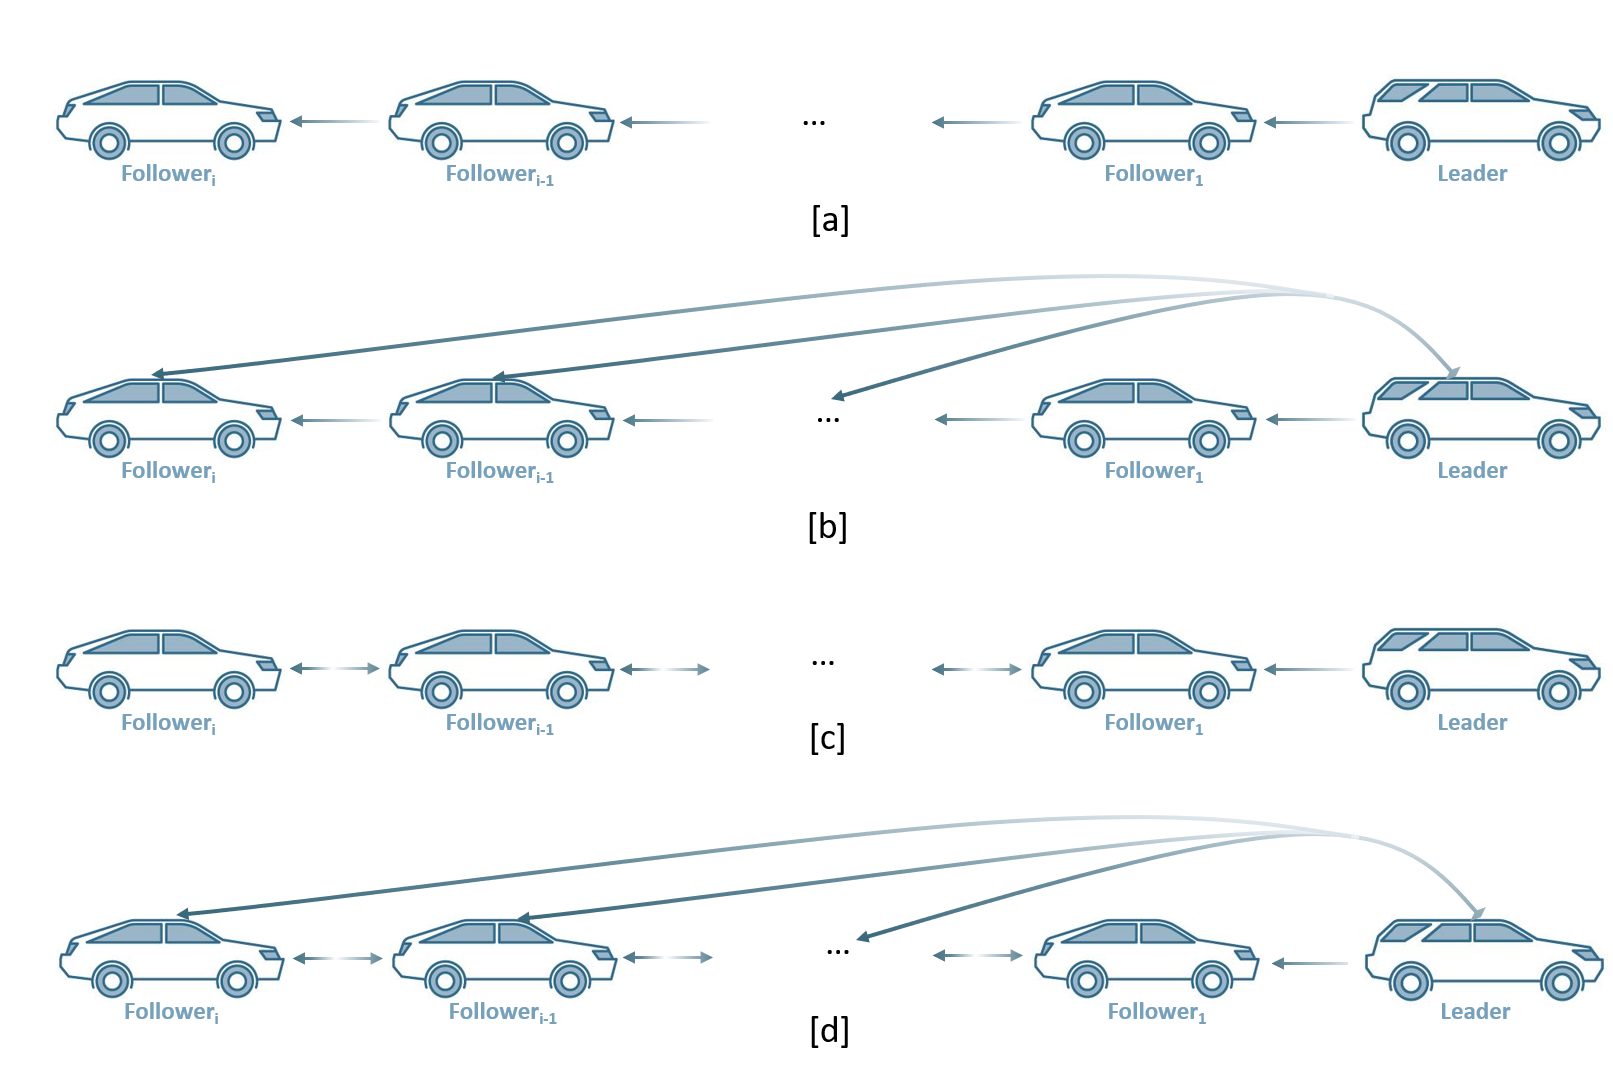
\includegraphics[width=11cm,height=18cm,keepaspectratio]{chapters/Chapitre_3/Figures/communication_topologies (1).png}
       % \vspace{-2.3mm}
        \caption{Communication topologies, adapted from \cite{ren2008distributed}}
        \label{fig:Communication topologies}
              %  \vspace{-5mm}
        \end{figure}

% c'est une excellente manière pour introduire la multi-behavior controler architecture ici enfaite ! 














     
     \subsection{Decision-making module} \label{sec: Decision-making} 
     The decision-making module derives its outcomes from a myriad of elements, including the assigned task, information regarding other vehicles within the MVS, acquired through the communication module (as discussed in Section \ref{sec: communication}), the environment's representation from the perception module (cf. Section \ref{sec: perception}), and the vehicle's position obtained from the localization module (cf. Section \ref{sec: localization}). 

    To illustrate, when a vehicle is navigating towards its designated goal and detects an obstacle in its path, the decision-making process comes into play. It must decide whether the vehicle should brake and come to a halt or maneuver to evade the obstacle, based on the vehicle's specific task and the overarching MVS objectives. 

    Various architectural frameworks have been devised to address these decision-making elements. One such framework is the LAAS architecture (An Architecture for Autonomy) \cite{alami1998architecture}, organized into three hierarchical levels: the decision level, the execution level, and the functional level. The decision level oversees processes requiring anticipation and a degree of global knowledge within the context of task execution. It encompasses planning and decision-making capacities. The execution level translates tasks into procedures composed of elementary robot actions and supervises their execution while reacting to the environment. The functional level comprises elementary robot functions implementing control loops. 

    Another architectural approach, especially suited for high-complexity navigation tasks, is the multi-controller (or behaviors) based decision architecture \cite{adouane2016autonomous}. This approach is founded on the concept that a robot can accomplish a complex global task through the coordination of several elementary behaviors/controllers, such as trajectory tracking, obstacle avoidance, and MVS coordination (e.g., splitting and joining), among others, to better govern the overall vehicle behavior \cite{adouane2016autonomous}. An example showcasing the use of this architecture approach is the hybrid multi-controller architecture proposed in \cite{ventura2015safe} (cf. Figure \ref{fig:Archi_Vilca} ) for a group of indoor robots. This architecture subdivides the overarching MVS navigation task into a set of accurate and dependable elementary controllers, such as obstacle avoidance, trajectory tracking, target reaching, and navigation in formation.  

\begin{figure}[!h]
        \centering 
        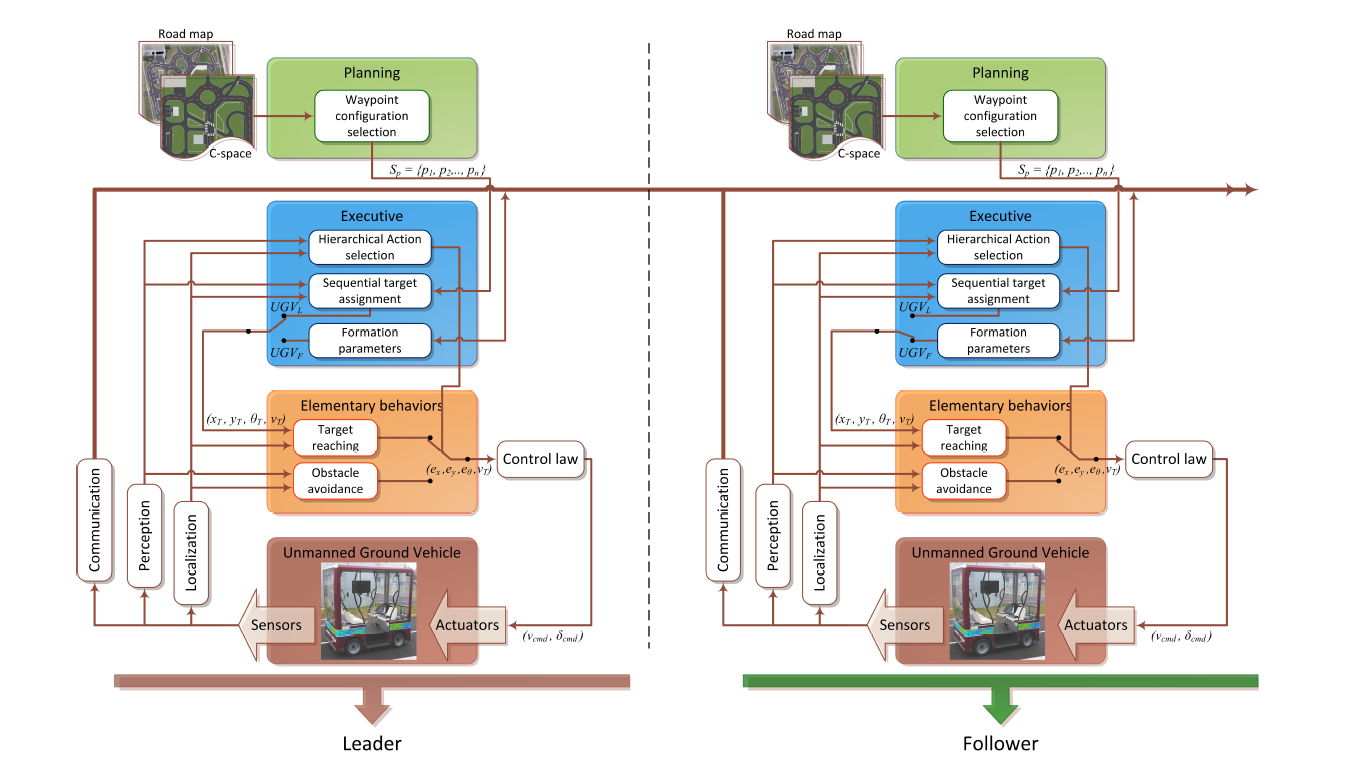
\includegraphics[width=13cm,height=20cm,keepaspectratio]{chapters/Chapitre_3/Figures/Archi_vilca}
        %\vspace{-2.3mm}
        \caption{Control architecture for the navigation in formation of MVS \cite{ventura2015safe}}
        \label{fig:Archi_Vilca}
            %    \vspace{-5mm}
        \end{figure}


      \subsection{Action module} \label{sec: Action} In the action module, the commands generated by the decision-making module (refer to Section \ref{sec: Decision-making}) are applied to the vehicle. A control law formulates these commands, instructing the actuators (motors) based on sensor information, the decision-making module (cf. Section \ref{sec: Decision-making}), and the vehicle's model. This control law's complexity can be tailored to align the system's modeling intricacies and the specific task at hand. 

   For example, in navigation applications, the design of the control law often focuses on guiding the vehicle along a predetermined trajectory, as demonstrated in \cite{vilca2015novel}\cite{chebly2019coupled}. Additionally, the control law can account uncertainties associated with the sensors and actuators, ensuring robust and dependable system operation \cite{yang2021comparative}.
    
   





















\subsection*{Discussion: MVS' technology future challenges}

Despite decades of research and development dedicated to MVS systems, there remains a significant untapped potential for technology to enhance the experience of road users. Nevertheless, MVS continue to grapple with a multitude of challenges, as outlined below \cite{eskandarian2019research}\cite{guanetti2018control}\cite{malik2021collaborative}\cite{ventura2015safe}: 

\textbf{Accurate perception/localization data:} Perception errors may be exacerbated in MVS. A data association mechanism that is efficient for a variety of vehicles and sensor designs is required \cite{kim2015impact}. The performance of the cooperative perception is highly dependent on the accuracy of relative localization. However, relative localization accuracy may be limited in particular circumstances \cite{luft2016recursive}. 

\textbf{Real-time coordination:} In scenarios featuring dynamic environments with multiple agents, ensuring system safety often hinges on cooperative motion planning for new maneuvers. This kind of planning relies heavily on the algorithms integrated on board and is particularly sensitive to the presence of nearby traffic. Consequently, achieving real-time coordination becomes imperative for the onboard controller \cite{ding2019rule}\cite{qu2009cooperative}. 

\textbf{Communication:} There is a notable absence of unified communication topologies and protocols tailored for the development of MVS \cite{hafner2021survey}. To address this challenge, a dependable decision/control strategy is needed to effectively manage various communication issues such as delays, packet losses, error messages, and interactions with uncooperative agents \cite{cui2019review}\cite{sun2021survey}. Furthermore, the efficiency of cooperative perception can be adversely affected by transmission latency and bandwidth limitations. The trade-off between communication bandwidth and maintaining optimal real-time closed-loop performance of the MVS has been a relatively under-explored aspect in this context \cite{ahmed2023vehicular}\cite{sarker2019review}\cite{daoud2023communication}.




\textbf{Accurate forecasts:} The lack of a unified communication protocol and a normalized decision/control architecture for MVS that facilitate access to more accurate predictions has led the majority of current methods to depend solely on static route information, like road curvature and speed limits. However, the potential of MVS often hinges on advancements in data forecasting, which is linked with central technological challenges. 

\textbf{Real-world verification:} The large majority of MVS related projects (e.g., CACC) were tested in a controlled environments (i.e., mainly due to local laws, on-road scenarios complexity, drivers acceptance, etc.)\cite{arvin2020safety}\cite{damaj2021connected}\cite{duboz2022exploring}. Thus, the MVS efficiency in dynamic and open on-road environments is difficult to know. Current verification issues for MVS' advanced algorithms include real-world testing and application to non-highway scenarios. 
 
% citer ce papier A review of connected and automated vehicle Platoon merging and splitting operations



Certainly, MVS have the potential to eliminate or greatly reduce unforeseen human errors by leveraging perception and localization sensors, as well as communication systems to enhance their awareness of the environment. These technologies offer substantial advantages in various scenarios, as discussed in the Section \ref{sec: CooperativeNavigation-Scenarios Overview} pertaining to CAV applications. However, realizing the full potential of MVS on public roads necessitates further exploration and utilization of these technologies. The decision and control mechanisms governing CAV systems should not solely rely on individual vehicle perceptions or objectives but should also consider the overall system state. A central challenge in the field of MVS navigation is the formulation of a robust control strategy. This strategy is a cornerstone in ensuring that all vehicles within the CAV system can seamlessly configure themselves in a synchronized and efficient manner to achieve their designated objectives. Additionally, by incorporating V2X communication, MVS can engage in the exchange of crucial data, as perception and localization information, as well as real-time status updates like intended acceleration, actual acceleration, or velocity, with fellow road users \cite{guanetti2018control}. An overview of MVS-related decision/control architecture will be discussed in the next section. 



%% architecture oriented 

\section{Overview of MVS control architecture} \label{sec:MVS_control_Architecture}
As depicted in Figure \ref{fig:MVS_architecture}, the MVS comprises multiple modules deployed within each AV part of the global ecosystem. Specifically, in this context, we are focusing on the MVS control architecture, encompassing system responsible for communication, perception, localization, decision-making/planning and control modules (cf. Figure \ref{fig:MVS_architecture}). The literature contains a plethora of descriptions regarding control architectures for MVS \cite{adouane2017toward}\cite{hichri2014cooperative}\cite{lozenguez2011map}\cite{vilca2016adaptive}\cite{assaad2018system}\cite{assaad2018cooperative}\cite{assaad2019autonomous}\cite{wang2019survey}.
%\cite{eskandarian2019research}
It is worth noting that this PhD thesis does not aim to provide an exhaustive classification of MVS structures and architectures. Nevertheless, a pivotal consideration that must be addressed before embarking on the development of the MVS decision/control architecture is the choice between a centralized and decentralized management scheme within the architectural framework \cite{7562449} \cite{rios2016automated}\cite{adouane2016autonomous}. This section is dedicated to evaluating the advantages and disadvantages of centralized vs. decentralized management within the MVS context. 

\begin{figure}[!h]
        \centering 
        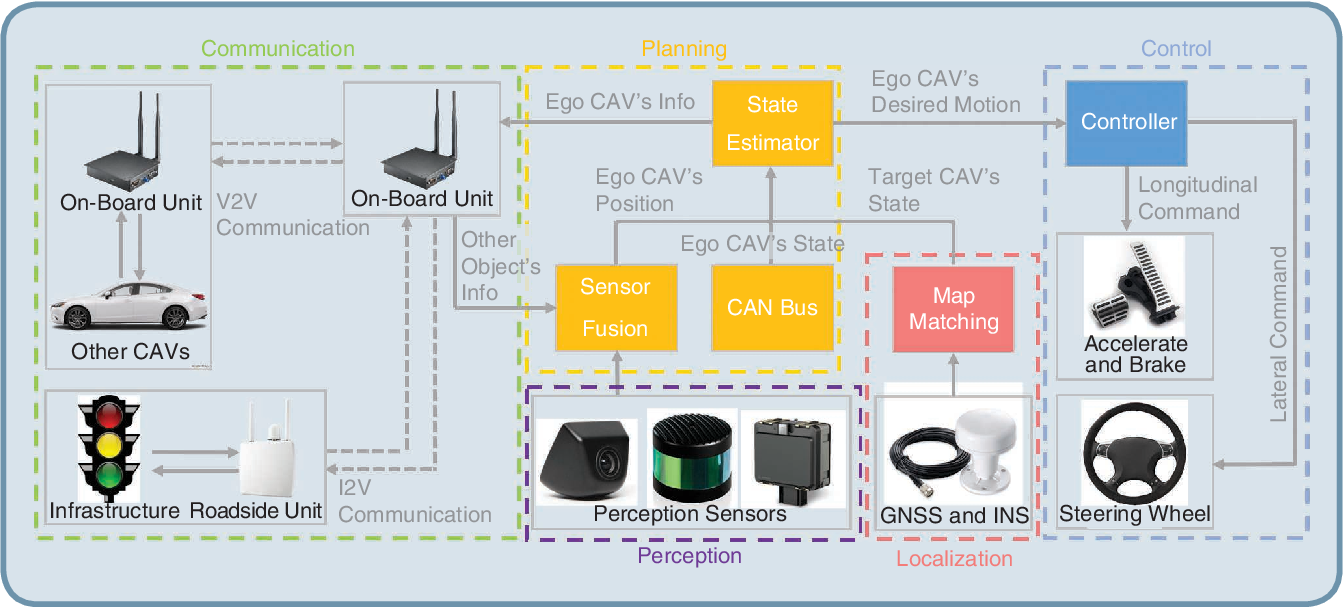
\includegraphics[width=12cm,height=18cm,keepaspectratio]{chapters/Chapitre_3/Figures/Architecture.png}
        %\vspace{-2.3mm}
        \caption{General cooperative architecture composed of: communication, perception, localization, planning and control modules \cite{wang2019survey}}
        \label{fig:MVS_architecture}
          %      \vspace{-5mm}
        \end{figure}
% voir dans les these encadrees par Reine si je trouve pas déja des définitions sur les architectures celle de rhada djaber je pense 

% ajouter les figures de chacune des architectures voir la these de vilca 
\subsection{Centralized approaches} \label{sec:CentralizedArchitecture}
An architectural configuration earns the designation of \textit{centralized}, when a portion or the entirety of the sensory and/or decision-making processes of individual robotic entities is detached from their physical structures and overseen by a central control unit \cite{diaz2016centralized}\cite{zhou2017stochastic}, commonly referred as a supervisor, or central planner \cite{adouane2016autonomous}. A centralized architecture is often synonymous of a Top-Down approach, which entails envisioning a conductor (the supervisor) orchestrating a group of mobile robots, akin to orchestra. 

The principal advantage of this architectural approach lies in the fact that a central unit, whether termed a controller or supervisor, can base its decisions on a comprehensive understanding of the entire system, which often surpasses the decision-making capacity of an individual component within the MVS \cite{khoshnevis1998centralized}. This paradigm is usually adopted in small-scale systems,
where the required computational capacity is moderate. Nevertheless, it is important to note that these architectures necessitate a complete awareness of every element within the system, demanding substantial computational power and a significant flow of information through extensive communication  \cite{khoshnevis1998centralized}\cite{yuta1992coordinating}. Additionally, they lack for robustness (due notably to its dependency on a single controller/ supervisor). 

Regarding the implementation, centralized architectures are designed to have the capacity to manage data originating from communication modules, perception/localization modules, and motion modules. This with the help of information flow topology \cite{zheng2015stability}, sensor fusion approaches \cite{gruyer2017perception}, and cooperative planning \cite{ren2008distributed}.

In scenarios where shared topological spaces are involved, such as intersection crossing, centralized approaches often emerge as viable solution when a limited number of intersecting vehicles is involved, in order to tackle the collision problem. In \cite{dresner2004multiagent}, the authors propose a reservation scheme as a means to oversee the control of a single intersection where two roads intersect. Thus, each vehicle is treated as a driver agent responsible for submitting a request to reserve specific space-time cells, allowing them to cross the intersection within a particular time interval. Upon receiving these reservation requests, the centralized reservation system takes decisions; accepting the request if there are no conflicts with previous accepted reservations, otherwise, the request is declined. With the development of the communication technologies such as 5G, centralized architectures gain a major popularity. However, its longer end-to-end latency prohibits its use in vehicle safety \cite{machardy2018v2x}. 

An example of centralized architecture is proposed in \cite{ventura2015safe}\cite{camacho2006roboskeleton}. This architecture named RoboSketon (cf. Figure \ref{fig:CentralizedArchitecture}) is based on three-layer architecture and it contains an agent that manages the other agents (cf. Figure \ref{fig:CentralizedArchitecture}). If the controlling agent (coachAgent) fails, the hole system could readily fail \cite{ventura2015safe}.  

\begin{figure}[!h]
        \centering 
        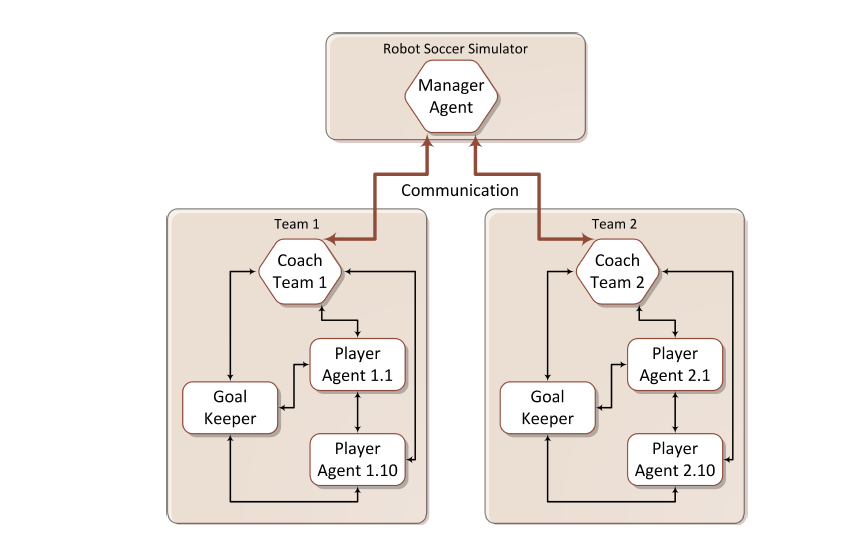
\includegraphics[width=11cm,height=18cm,keepaspectratio]{chapters/Chapitre_3/Figures/CentralizedArchitecture}
        %\vspace{-2.3mm}
        \caption{Example of centralized architecture \cite{ventura2015safe}\cite{camacho2006roboskeleton}}
        \label{fig:CentralizedArchitecture}
               % \vspace{-5mm}
        \end{figure}

\subsection{Decentralized approaches}\label{sec:DecentralizedArchitecture}
A decentralized architecture is a system in which parts have local authorities by themselves \cite{assaad2019overview}. In contrast to the centralized architecture, in a decentralized architecture, each vehicle within the MVS maintains its own independent processes for perception/localization and decision-making/planning. Such architectures entail a reduction in the volume of communicated signals and data. Notably, in this decentralized setup, each vehicle within the MVS does not require a comprehensive understanding of the overall environment prior to taking actions within its immediate surroundings. 

One of the key advantages of this decentralized design is that the AVs within the MVS paradigm can individually control their operations without necessitating external commands, which impacts resilience if the system faces defects and failures. Moreover, decentralized control facilitates parallel computation, enhancing system responsiveness and thereby ensuring the reliability and scalability of the implementation  \cite{cao1997cooperative}\cite{feddema2002decentralized}\cite{ren2008distributed}. The primary drawback of decentralized management lies in its heavy reliance on extensive coordination. This is primarily because the specific tasks allocated to each vehicle are embedded within their local control systems. Consequently, if there is a need to alter the assigned tasks, achieving a global reconfiguration of the MVS without the presence of a supervisor can be a challenging endeavor. 

The decentralization paradigm can also be applied to various aspects of the MVS, including communication technologies \cite{abboud2016interworking}\cite{ghosal2020security}, perception techniques involving decentralized fusion \cite{winner2014handbook}, and cooperative motion planning \cite{7562449}. Additionally, in the context of road safety, decentralized systems like dedicated short-range communication have demonstrated their advantages when compared to cellular network like 5G \cite{jurgen2012v2v}\cite{harding2014vehicle}. The decentralization paradigm when well mastered is more flexible to deal with MVS having a large number of entities and is generally a synonym of Bottom-Up approach \cite{adouane2005architectures}. 

A typical example is the ALLIANCE/L-ALLIANCE architecture developed in \cite{parker1994alliance}\cite{parker1996alliance}\cite{parker1998alliance} (cf. Figure \ref{fig:DecentralizedArchitecture}) for heterogeneous robots. Robots have information about their actions and the actions of the group through the top-board communication topology. This architecture uses behavior-based controllers which depend on the assigned robot's task. L-Alliance \cite{parker1996alliance} is an extension of the Alliance architecture \cite{parker1994alliance} which uses reinforcement learning to adjust the activation parameters of the behaviors \cite{ventura2015safe}. 

% ajouter un footnote avec la définition de bottom up and top down voir la these de lounis.

\begin{figure}[!h]
        \centering 
        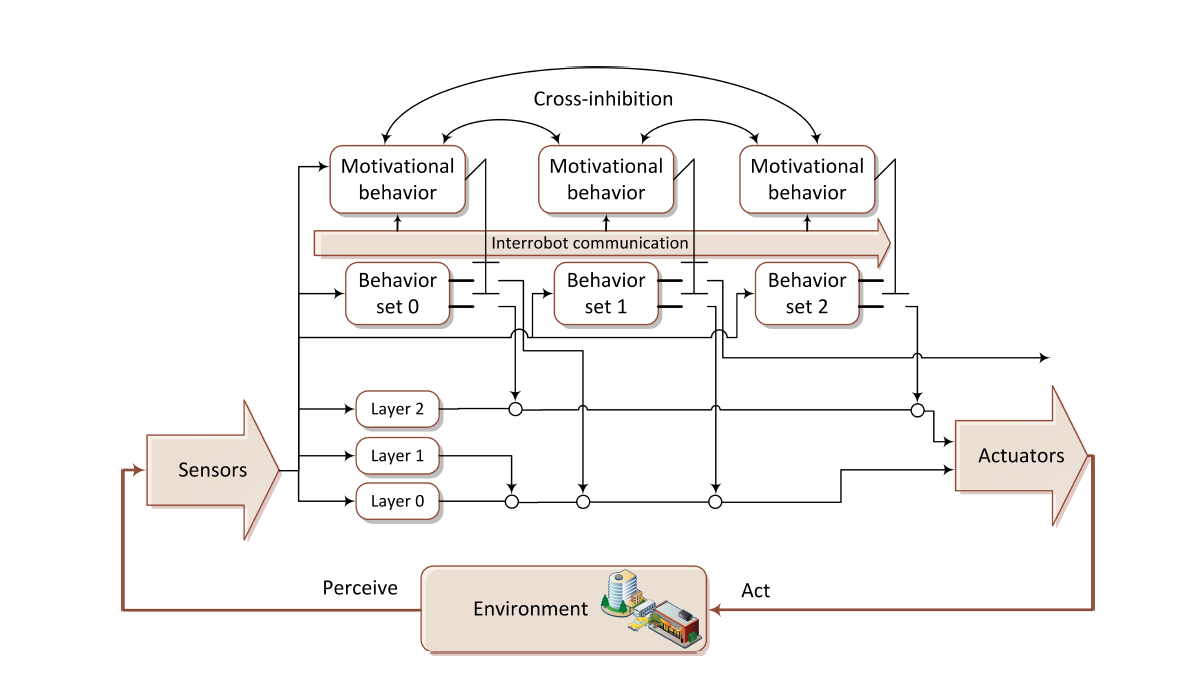
\includegraphics[width=11cm,height=18cm,keepaspectratio]{chapters/Chapitre_3/Figures/Decentralized}
       % \vspace{-2.3mm}
        \caption{Example of decentralized architecture \cite{ventura2015safe}\cite{parker1998alliance}}
        \label{fig:DecentralizedArchitecture}
             %   \vspace{-5mm}
        \end{figure}


\newpage


\subsection{Hybrid approaches}
% hybride architectures 
% Hierarchical architecture 
Other comprehensive studies with similar discussion suggesting some variations in control approach/architectures might also be discovered in \cite{chen2017towards}\cite{evestedt2016interaction}\cite{jiang2017eco}\cite{pendleton2017perception}\cite{yurtsever2020survey}\\ \cite{loke2019cooperative}\cite{zhou2016impact}. It is proposed to highlight several types of notable control architectures as follows: 

\begin{itemize}



\item \textbf{Hierarchical architecture:} This type of control architecture exhibits a form of local centralization, as discussed in \cite{ren2008distributed}\cite{adouane2006behavioral}\cite{assaad2019overview}, while maintaining decentralization in a global context. To clarify further, each vehicle within this framework independently manages its assigned responsibilities but provides updates to a central planner part of the vehicle's architecture regarding the status of its activities. Based on this definition, it becomes evident that the vast majority of MVS are structured hierarchically, as elucidated in \cite{girard2001overview}\cite{karagiannis2011vehicular}. This hierarchical structuring is particularly well-suited for large-scale designs, where the overarching task is subdivided into a series of smaller, more manageable sub-problems, each addressed within distinct layers \cite{varaiya2000question}. 

An illustrative example of this architectural structuring is found in the UM-PRS (University of Michigan Procedural Reasoning System) \cite{lee1994prs}\cite{lee1999reactive}, where a multi-agent system is employed for environmental recognition. 








%%%
\item \textbf{Hybrid Centralized/Decentralized architecture}: This control framework combines a high-level central controller with localized decentralized controllers within individual vehicles \cite{assaad2019overview}\cite{noreils1993toward}\cite{siciliano2008springer}\cite{ventura2015safe}. Consequently, this design combines both of the noteworthy advantages of the centralized architecture (cf. Section \ref{sec:CentralizedArchitecture}) and the decentralized architecture (cf. Section \ref{sec:DecentralizedArchitecture}): 
\begin{enumerate}
    \item Centralized planner: The centralized planner assumes a pivotal role as a high-level controller overseeing the vehicles within the MVS. 

    \item Robustness: The decentralized controllers within the vehicles part of the MVS exhibit fault tolerance, enhancing the system's robustness. 

    \item Flexibility: The hybrid architecture provides the flexibility to adjust the global task or control strategy based on inputs from both the centralized and decentralized control components. 
\end{enumerate}

One compelling illustration of this architecture's application is its use in MVS navigation in formation, with a primary focus on safety and flexibility. The centralized approach allows to the central entity (leader of the formation) to manage the configuration desired formation even for formation reconfiguration. The decentralized approach allows each robot (follower) locally generate its commands to track its assigned target \cite{ventura2015safe}. 

One example of the centralized/decentralized architecture is proposed in \cite{simmons2001first} (cf. Figure \ref{fig:CentralizedDecentralizedArchitecture}). It is based on three-layer architecture, and it allows coordination between the robots (communication layer) and autonomy in action (executive and behavioral layer) \cite{ventura2015safe}\cite{simmons2001first}. 
    
\end{itemize}

\textbf{\begin{figure}[!h]
        \centering 
        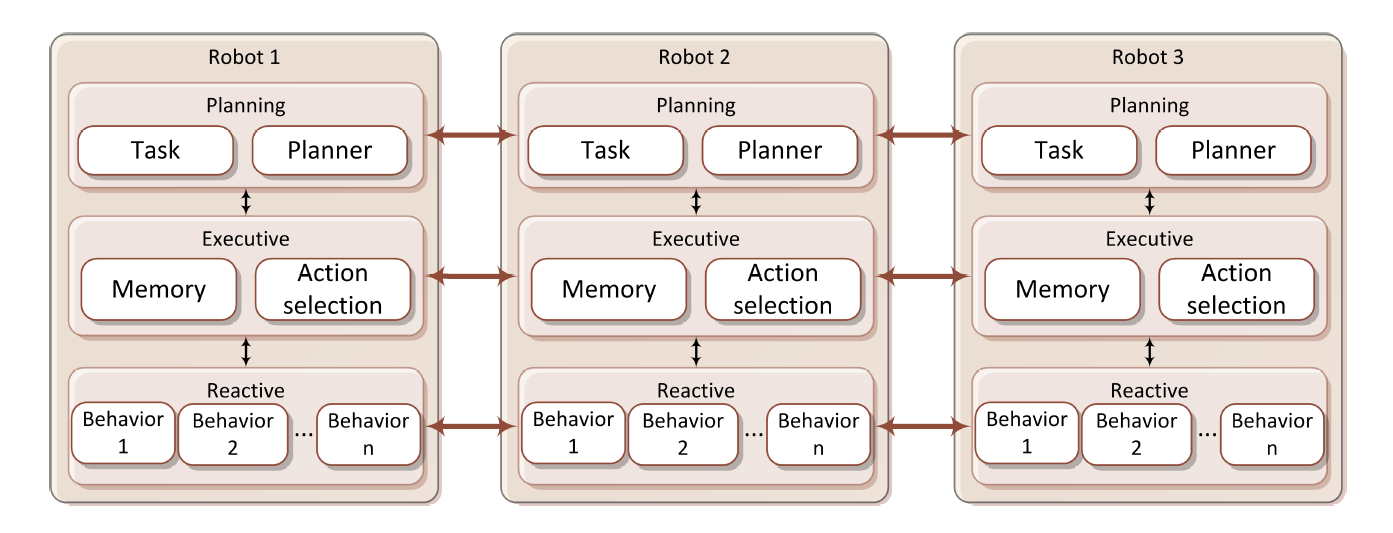
\includegraphics[width=11cm,height=18cm,keepaspectratio]{chapters/Chapitre_3/Figures/Centralized-Decentralized}
        %\vspace{-2.3mm}
        \caption{Example of centralized/decentralized architecture \cite{ventura2015safe}\cite{simmons2001first}}
        \label{fig:CentralizedDecentralizedArchitecture}
                %\vspace{-5mm}
        \end{figure}}

% Nous, on propose quoi ? 

\newpage
The central aim of this Ph.D. thesis revolves around the creation of a Decision/Control architecture that mitigates in-between the advantages of both the centralized and the decentralized framework (cf. Table \ref{Tab:CentralizedVsDecentralized}).  Designed for cooperative based maneuvers (cf. Section \ref{sec: CooperativeNavigation-Scenarios Overview}), the MVS targeted architecture aims to seamlessly align with the individual control architectures of the vehicles part of the MVS, while the Decision/Control architecture for MVS consistently leans toward a bottom-up strategy, where decentralized modules are in charge of performing local tasks. There are specific scenarios or tasks where leveraging global knowledge from a central planner can enhance MVS performance. 

\begin{table}[!h]
\
\caption{Comparison between MVS architectures \cite{adouane2005architectures}}\label{Tab:CentralizedVsDecentralized}
  \begin{adjustwidth}{-0.10\textwidth}{-0.10\textwidth}

\begin{tabular}{|l|llll|}
\hline
              & \multicolumn{1}{l|}{Perception}                                          & \multicolumn{1}{l|}{Localization}                                          & \multicolumn{1}{l|}{Decision}                                          & Action                                                                                               \\ \hline
Centralized   & \multicolumn{3}{l|}{\begin{tabular}[c]{@{}l@{}}A central entity uses the information \\ from all the deported sensors to unde-\\ strand the robots' environment and to \\ compute the commands to send to them.\end{tabular}} & \begin{tabular}[c]{@{}l@{}}Each robot executes the \\ command sent by the central \\ entity.\end{tabular} \\ \hline
Decentralized & \multicolumn{4}{l|}{\begin{tabular}[c]{@{}l@{}}Each robot uses local information from its sensors to understand its \\ environment and to generate and execute its commands to accomplish \\the assigned task.\end{tabular}}                                                                                                               \\ \hline
\end{tabular}
  \end{adjustwidth}

\end{table}

%% methodologie oriented 


% TODOD list ---> il faut charcher un angle d'attaque pour introduire les différentes méthodologies -- peut etre revenir à l'introduction et fragmenter encore plus l'architecture pour avoir d'information 
% il faut introduire la notion de la réactivité et la congnivité 
% il faut préciser plus d'info sur les différents blocks qui font l'arhitecture et les associers aux notions de réactivité etc 
% il faut parler des méthodologie, 








\section{MVS navigation in formation: a review} \label{sec: formation_control_theory}
% le but ici est de detailler les differents types et formalisme qui existe pour le définition de la formation
% donc, ca va parler de la structure virtuelle, du leader follower, etc. 






Numerous research laboratories, including the current thesis work, have directed their focus toward applications involving navigation in formation. These applications find utility across a spectrum of domains, spanning transportation, agriculture, and military applications \cite{ventura2015safe}\cite{wolterink2011automated}\cite{meyer2014research}. 

Formation control, at its core, pertains to the capacity to maintain the relative positions of a group of vehicles/robots with respect to each others or to a specific reference. In essence, this entails ensuring that the group of vehicles or robots adheres to a predefined geometric formation \cite{adouane2016autonomous}.

Navigating MVS in formation presents a set of intricate challenges, as highlighted in \cite{ventura2015safe}. These challenges encompass fundamental questions: 

\begin{itemize}
    \item \textbf{Defining the desired formation:} What configuration should the MVS aims to achieve? 
    \item \textbf{Determining actual positions:} How do the individual vehicles ascertain their current positions within the formation? 
    \item \textbf{Maintaining formation:} What strategies do the vehicles employ to ensure the formation remains intact? 
    \item \textbf{Adapting to Road Conditions and Obstacles:} How can the MVS adapt to varying road topologies and the presence of obstacles? 
    \item \textbf{Evaluating formation performance:} What criteria are employed to assess the performance of the MVS formation? 
\end{itemize}

To address these questions, various approaches have been developed, including Leader-Follower, Virtual Structure, Behavior-based, and other Optimization-based techniques \cite{chen2005formation}\cite{murray2007recent}, each offering insights into the complexities of formation navigation within MVS.

\subsection{Leader-Follower} \label{sec: Leader-follower}
% il faut ajouter une section CACC


The concept of leader-follower formation approach involves a hierarchical structure, comprising a single vehicle designated as the leader ($UGV_L$), while the rest, referred as the followers ($UGV_i$ and $UGV_j$), determine their positions relative to the leader pose or another reference pose (cf. Figure \ref{fig:Leader_follower}). They achieve this by utilizing their representation of the environment from their own positions \cite{ventura2015safe}\cite{michaud2002distributed}\cite{el2012echelon}.



\textbf{\begin{figure}[!h]
        \centering 
        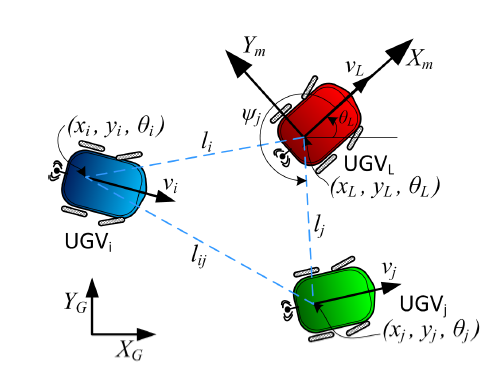
\includegraphics[width=9cm,height=18cm,keepaspectratio]{chapters/Chapitre_3/Figures/Leader_follower.PNG}
        %\vspace{-2.3mm}
        \caption{The leader follower formation modeling approach \cite{ventura2015safe}}
        \label{fig:Leader_follower}
               % \vspace{-5mm}
        \end{figure}}


In the realm of transportation, a prevalent application of this formation strategy is the one-dimensional leader-follower, often referred to as platooning-based formation or column formation. In this context, a leader assumes a pivotal role within the MVS formation, tasked with following a reference trajectory while simultaneously serving as the guiding reference for the followers. The followers, in turn, closely track the leader's or another guide's position and adapt their control inputs accordingly. This leader-follower can be characterized by either constant spacing or constant headway, as it can be seen in Cooperative Adaptive Cruise Control (CACC) (cf. Section \ref{sec: CACC}), among other leader-follower models found in the literature, such as the spring-damper system \cite{hutchison_bending_2009}. The spring-damper model introduces one or more interaction models, enabling control over the inter-vehicle distances within the MVS formation (cf. Figure \ref{fig:SpringDamper}). 

One notable advantage of the leader-follower approach is its compatibility with the decentralized architecture, wherein each vehicle autonomously makes decisions based on local information in relation to a common reference, thereby maintaining the formation's shape. Control techniques rooted in optimal control or model predictive control can be leveraged to uphold the formation shape. In \cite{7225700}, an exhaustive survey of methods employed to ensure the effectiveness of the leader-follower approach is given. 

However, this approach has its limitations. It heavily relies on the leader, rendering it susceptible to faults in the leader vehicle. Any issues with the leader can disrupt the entire navigation task or even lead to collisions within the MVS formation. Furthermore, when dealing with large MVS formations, where the leader is responsible of supervising the followers, significant computational costs arise, and communication issues, such as package losses and delays, can become prominent concerns. 







\textbf{\begin{figure}[!h]
        \centering 
        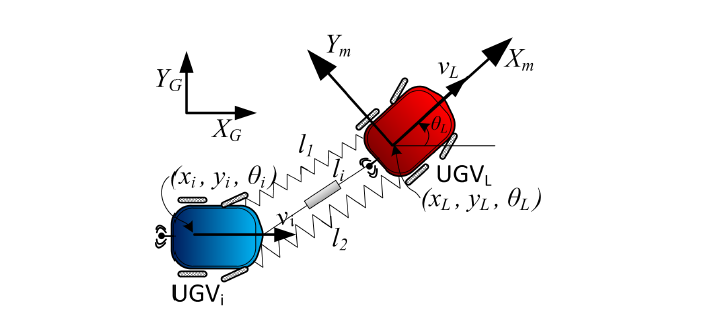
\includegraphics[width=10cm,height=18cm,keepaspectratio]{chapters/Chapitre_3/Figures/Virtual_Structure}
      %  \vspace{-2.3mm}
        \caption{Leader-follower based on spring damper system \cite{ventura2015safe}}
        \label{fig:SpringDamper}
               % \vspace{-5mm}
        \end{figure}}


\subsection{Virtual Structure} \label{sec: Virtual-structure}


A vehicle formation materializes when multiple vehicles collaborate across multiple lanes while adhering to a pre-defined configuration. To govern such formations, the virtual structure has been adopted, effectively dividing the formation control into a high-level virtual structure and a low-level control problem  \cite{7535413}. \\

This approach can be summarized through the following steps \cite{yang_quan_chen_formation_2005}: 
\begin{enumerate}
    \item \textbf{Defining the virtual rigid body:} The dimension, shape, and dynamics of a virtual rigid body are defined based on the number of vehicles and the road geometry (cf. Figure \ref{fig:Virtual_Structure}). 

    \item \textbf{Vehicle tracking: } Each vehicle within the MVS closely tracks its designated virtual agent or target (cf. Figure \ref{fig:Virtual_Structure}). 

    \item \textbf{Virtual agent motion}: The motions of the virtual agent or target are computed to align with the desired maneuver. 
\end{enumerate}
\textbf{\begin{figure}[!h]
        \centering 
        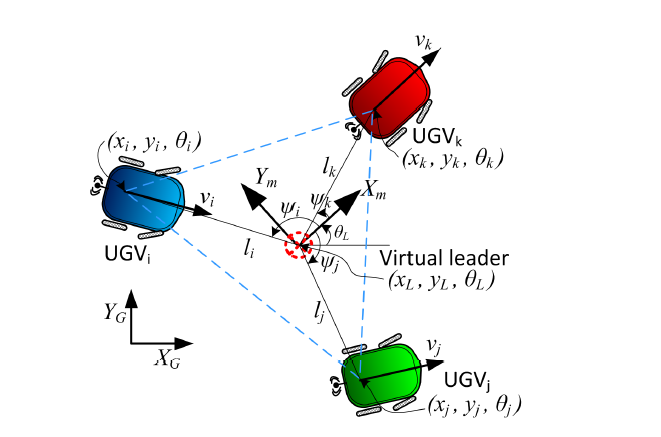
\includegraphics[width=10cm,height=18cm,keepaspectratio]{chapters/Chapitre_3/Figures/Virtual_Structure_Corrected.PNG}
       % \vspace{-2.3mm}
        \caption{Virtual structure formation modeling approach \cite{ventura2015safe}}
        \label{fig:Virtual_Structure}
          %      \vspace{-5mm}
        \end{figure}}



The advantages of the virtual structure approach primarily stem from its simplicity compared to other formation control methods. It also offers flexibility in shaping different types of formation control \cite{4651041}\cite{benzerrouk:tel-00669559}\cite{2014_Benzerrouk_RAS}. Some research combines the leader-follower approach with a deformable  virtual structure to tackle formation reconfiguration \cite{8430659} (cf. Figure \ref{fig:Archi_Vilca}). Formal safety guaranteed for the entire fleet is provided by employing a reconfiguration matrix that considers inter-vehicle distances to prevent collisions \cite{8430659} \cite{ventura2015safe}. 

However, there are drawbacks associated with the virtual structure approach, mainly linked to its centralized nature. The central unit is responsible of assigning virtual agents/nodes and overseeing formation maintenance. Additionally, factors like road shape and vehicle dimensions must be taken into account.




\subsection{Behavior-based}
Formation control using a behavior-based approach involves the task of decomposing the main objective into several fundamental sub-tasks (cf. Figure \ref{fig:Behavior-based}), with the ultimate aim of generating the desired emergent behavior \cite{arkin1998behavior}. The selection of these sub-tasks is carried through two primary methods: 

\begin{itemize}
    \item \textbf{Competitive selection:} In this method, only one behavior is chosen at any given time. The design of such a selection system follows a hierarchical structure, with the desired behavior holding the highest priority compared to others (cf. Figure \ref{fig:Behavior-based}). It is worth noting that architectures employing hierarchical selection may encounter challenges in stability analysis during the switching phase \cite{adouane2016autonomous}. 

    \item \textbf{Cooperative selection:} In contrast to the competitive selection, the cooperative selection in Figure \ref{fig:Behavior-based} allows for the simultaneous selection of two or more behaviors, which are then fused to create an emergent complex behavior. While this approach offers the potential to achieve sophisticated behaviors \cite{adouane2016autonomous}, it introduces complexities during the transition phase what can be a challenging task \cite{SCHONER1995213}. 
    
\end{itemize}

The primary advantage of the behavior-based approach is its adaptability to handle more complex tasks and its capacity to generate emergent behaviors. Some research work has successfully integrated graph theory into behavior-based formation control to address issues associated with time-varying communication \cite{4522625}. Another proposed formation control architecture based on selection of behaviors, combining both self-centered maneuvers through competitive selection and more altruistic maneuvers with the assistance of cooperative selection is presented in \cite{736776}. 


\begin{figure}[!h]
        \centering 
        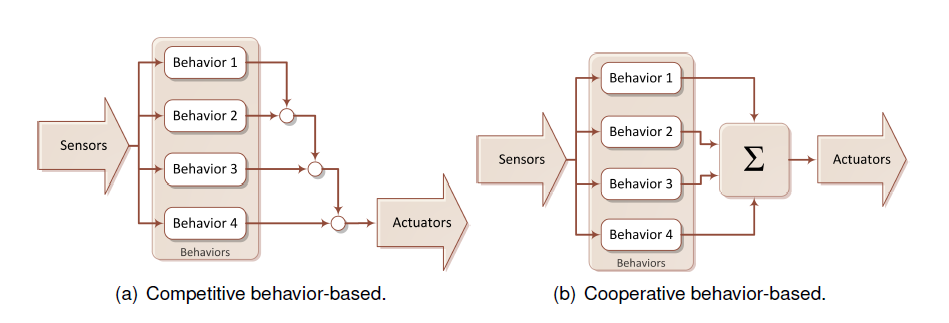
\includegraphics[width=14cm,height=18cm,keepaspectratio]{chapters/Chapitre_3/Figures/behavior_based.PNG}
       % \vspace{-2.3mm}
        \caption{Behavior-based formation modeling approach \cite{ventura2015safe}}
        \label{fig:Behavior-based}
          %      \vspace{-5mm}
        \end{figure}



\newpage

\subsection{Consensus-based control} \label{sec:consensus_control}

In the realm of MVS, consensus-based control represents an important and fundamental part of the literature related to formation control \cite{ren2008distributed}. Thus, consensus-based control is part of the MVS control architecture paradigm (cf. Section \ref{sec: MVS_control_Architecture}), especially, decentralized MVS control architecture (cf. Section \ref{sec:DecentralizedArchitecture}). The essence of consensus-based control lies in the convergence of individual entities toward a common objective through interactions facilitated by sensing and communication networks (cf. Figure \ref{fig:consensus_control}), as elaborated in Section \ref{sec: communication}. 

The formation modeling used part of the consensus-based control theory relies on the algebraic graph topology as in Figure \ref{fig:consensus_control}, where the vehicles are represented by the nodes and in-between node links are the vehicle's in-between communication. The primary objective of consensus-based control is to stabilize the relative distances or headway between vehicles in the MVS to achieve predefined task. Formation control, in essence, plays an important role in realizing consensus-based control, as it governs the spacial configuration and relative positions of the MVS vehicle, contributing to the fulfillment of a shared goal \cite{ren2008distributed}\cite{ma2017consensus}\cite{gao2022survey}.






In \cite{4283094}, a first order consensus-based protocol was implemented. This entailed the utilization of a decentralized control framework built upon the leader-follower formation approach, ensuring the formation maintenance through information exchange among neighboring vehicles. Additionally, in \cite{6891349}, a control algorithm rooted in consensus-based control was proposed, accounting for communication delays to govern a platoon-based formation. The stability of this formation was mathematically proven using the Lyapunov formalism \cite{khalifa2019vehicles}\cite{khalifa2018vehicles}. In this approach, the leader disseminates its state information, while each follower solely measures its relative position w.r.t. the preceding vehicle part of the MVS. This localized approach to formation maintenance was integrated with consensus-based control, even accommodating network and sensor time delays as well as variable leader velocities. Conditions ensuring both internal and string stability of the platoon were established. 


Consensus-based control enables the formal modeling of formations by integrating the control of vehicles and the MVS communication topology. Nevertheless, consensus-based control does entail certain drawbacks. For instance, it often simplifies the dynamics of the MVS vehicles by treating them solely as integrators \cite{ren2008distributed}. Furthermore, consensus-based control theory relies on the assumption of continuous connectivity among the vehicles to establish a strongly connected graph, which might not always hold in practice \cite{wang2022consensus}. 







\begin{figure}[!h]
        \centering 
        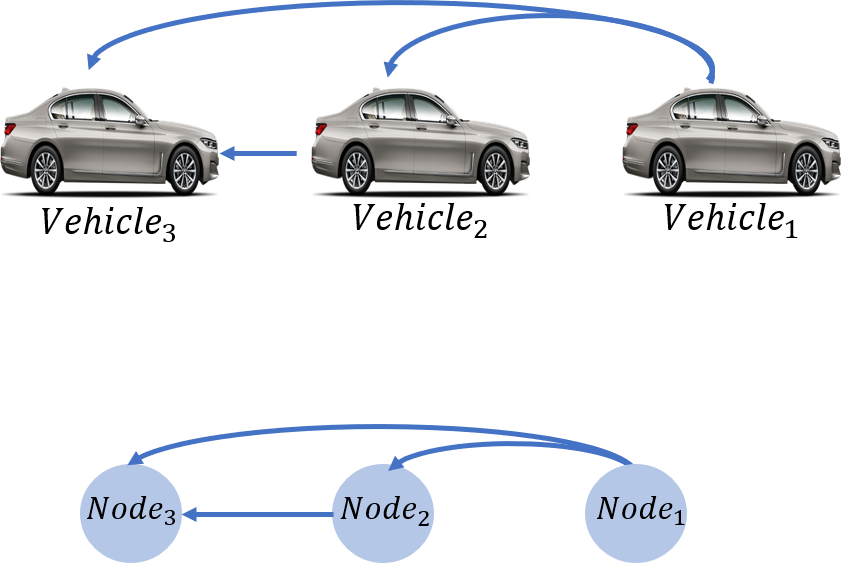
\includegraphics[width=9cm,height=18cm,keepaspectratio]{chapters/Chapitre_3/Figures/Consensus_control.png}
       % \vspace{-2.3mm}
        \caption{From communication topology to algebraic graph representation for consensus-based control}
        \label{fig:consensus_control}
          %      \vspace{-5mm}
        \end{figure}

\subsection{Discussion} \label{sec: Disc_formation_approach}

It is evident that the primary focus of the literature on MVS formation control has predominantly revolved around platooning-based formations. Approaches such as leader-follower paradigm (cf. Section \ref{sec: Leader-follower}) have been extensively employed to tackle various challenges, including platooning modeling \cite{li2022platoon}, string stability (ensuring the stability of the platoon)\cite{feng2019string}, and information flow \cite{ren2008distributed}, among others. 

However, the leader-follower approach exhibits certain limitations, particularly in flexibility and adaptability, when dealing with what we refer to as \textit{challenging scenarios}, such as intersection crossings or on-ramp merging (as discussed in Section \ref{sec: Leader-follower}). To mitigate these limitations, exploring the virtual structure approach (cf. Section \ref{sec: Virtual-structure}) emerges as a potential solution, with a clear imperative for tailored adaptations to suit on-road contexts. 

On the other hand, behavior-based formation modeling and control may find its application in scenarios where the main task can be easily divided, and a common goal is distinctly identified by the formation's agents. This approach typically relies on a central entity to define task decomposition and distribution among agents. However, to circumvent the drawbacks of centralization, our work endeavors to promote decentralized approaches. 

Consensus-based control offers the advantage of formally modeling formation structures. However, its dependence on the assumption of a strongly connected graph makes it less fault-tolerant, particularly in dynamic environments such as highway scenarios. 

Clearly, our literature review has indicated that on-road formation-based approaches have not significantly explored the applications of the virtual structure approach. While this approach may initially seems conceptual, we intend to delve into this topic further in Chapter \ref{Chap03} to explore its feasibility and applications. 



\section{MVS Navigation in complex environments} \label{sec:review_MVS_application}
As previously discussed in Section \ref{sec: CooperativeNavigation-Scenarios Overview}, and as evident from the literature review, the coordination challenges within MVS extend to both rural (cf. Figure \ref{fig:rural}) and urban settings. These challenges encompass a range of scenarios, including highway speed coordination (cf. Figure \ref{fig:Highway_navigation}), merging onto on-ramps and off-ramps (cf. Figure \ref{fig:on-ramp_highway}), and coordination intersections (cf. Figure \ref{fig:intersection_urban}) \cite{bernardin2019scenario}\cite{guo2019urban}\cite{wang2019survey}\cite{7562449}.  Additionally, MVS planning technology, known for its substantial impact on road capacity \cite{amoozadeh2015platoon}\cite{zhao2013simulation}, has gained significant attention over the past decade. Furthermore, a majority of fundamental research efforts have concentrated on MVS highway speed harmonization \cite{hegyi2005optimal}\cite{papageorgiou2008effects}\cite{ma2016freeway}\cite{talebpour2013speed}, as it holds the potential to reduce overall times and average energy consumption \cite{VAHIDI2018822}. 

% \textbf{\begin{figure}[!h]
%         \centering 
%         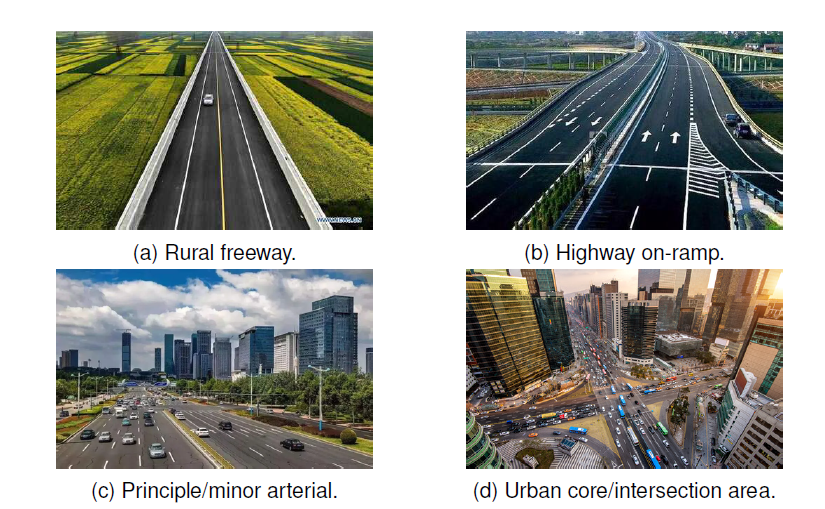
\includegraphics[width=11cm,height=18cm,keepaspectratio]{chapters/Chapitre_3/Figures/Scenarios}
%         \vspace{-2.3mm}
%         \caption{\cite{zhu2022hierarchical}}
%         \label{fig:Scenarios}
%                 \vspace{-5mm}
%         \end{figure}}





\begin{figure}[ht]
\begin{minipage}[b]{0.45\linewidth}
\centering
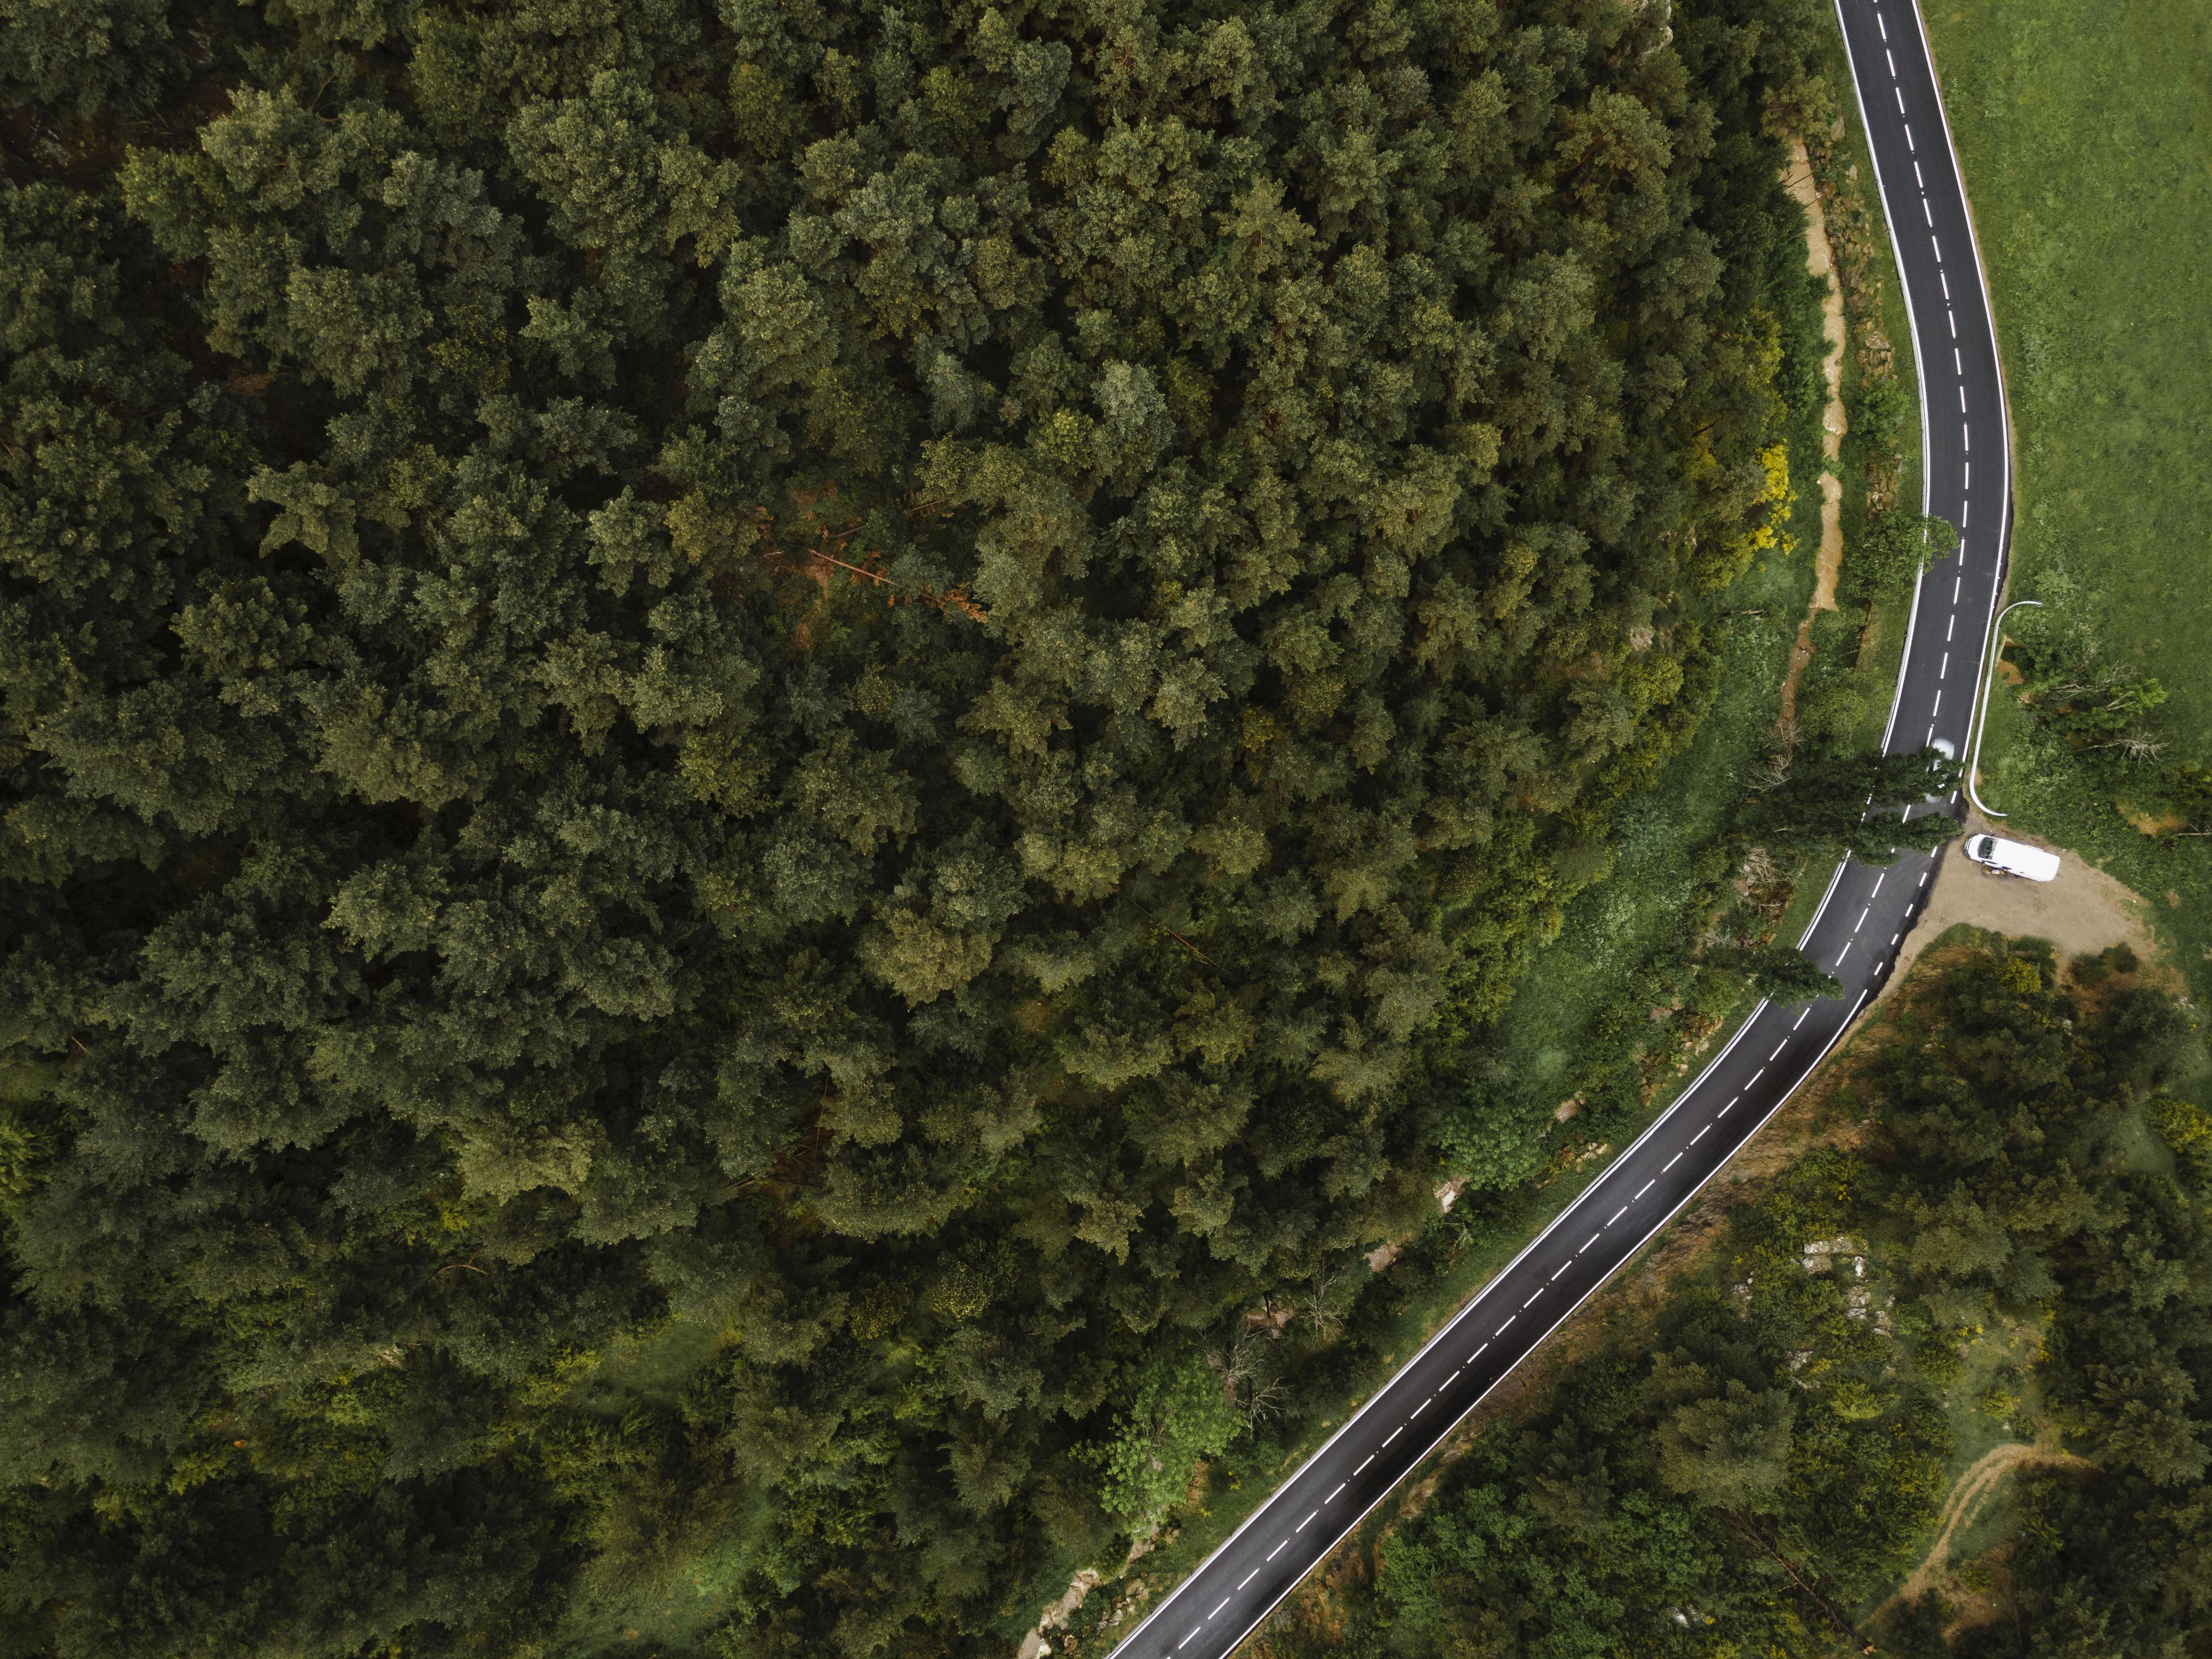
\includegraphics[width=\textwidth]{chapters/Chapitre_3/Figures/rural.jpg}
\caption{Rural freeway}
\label{fig:rural}
\end{minipage}
\hspace{0.5cm}
\begin{minipage}[b]{0.45\linewidth}
\centering
\includegraphics[width=5.8cm,height=4.35cm]{chapters/Chapitre_3/Figures/intersection.jpg}
\caption{Intersection crossing}
\label{fig:intersection_urban}
\end{minipage}

\begin{minipage}[b]{0.45\linewidth}
\centering
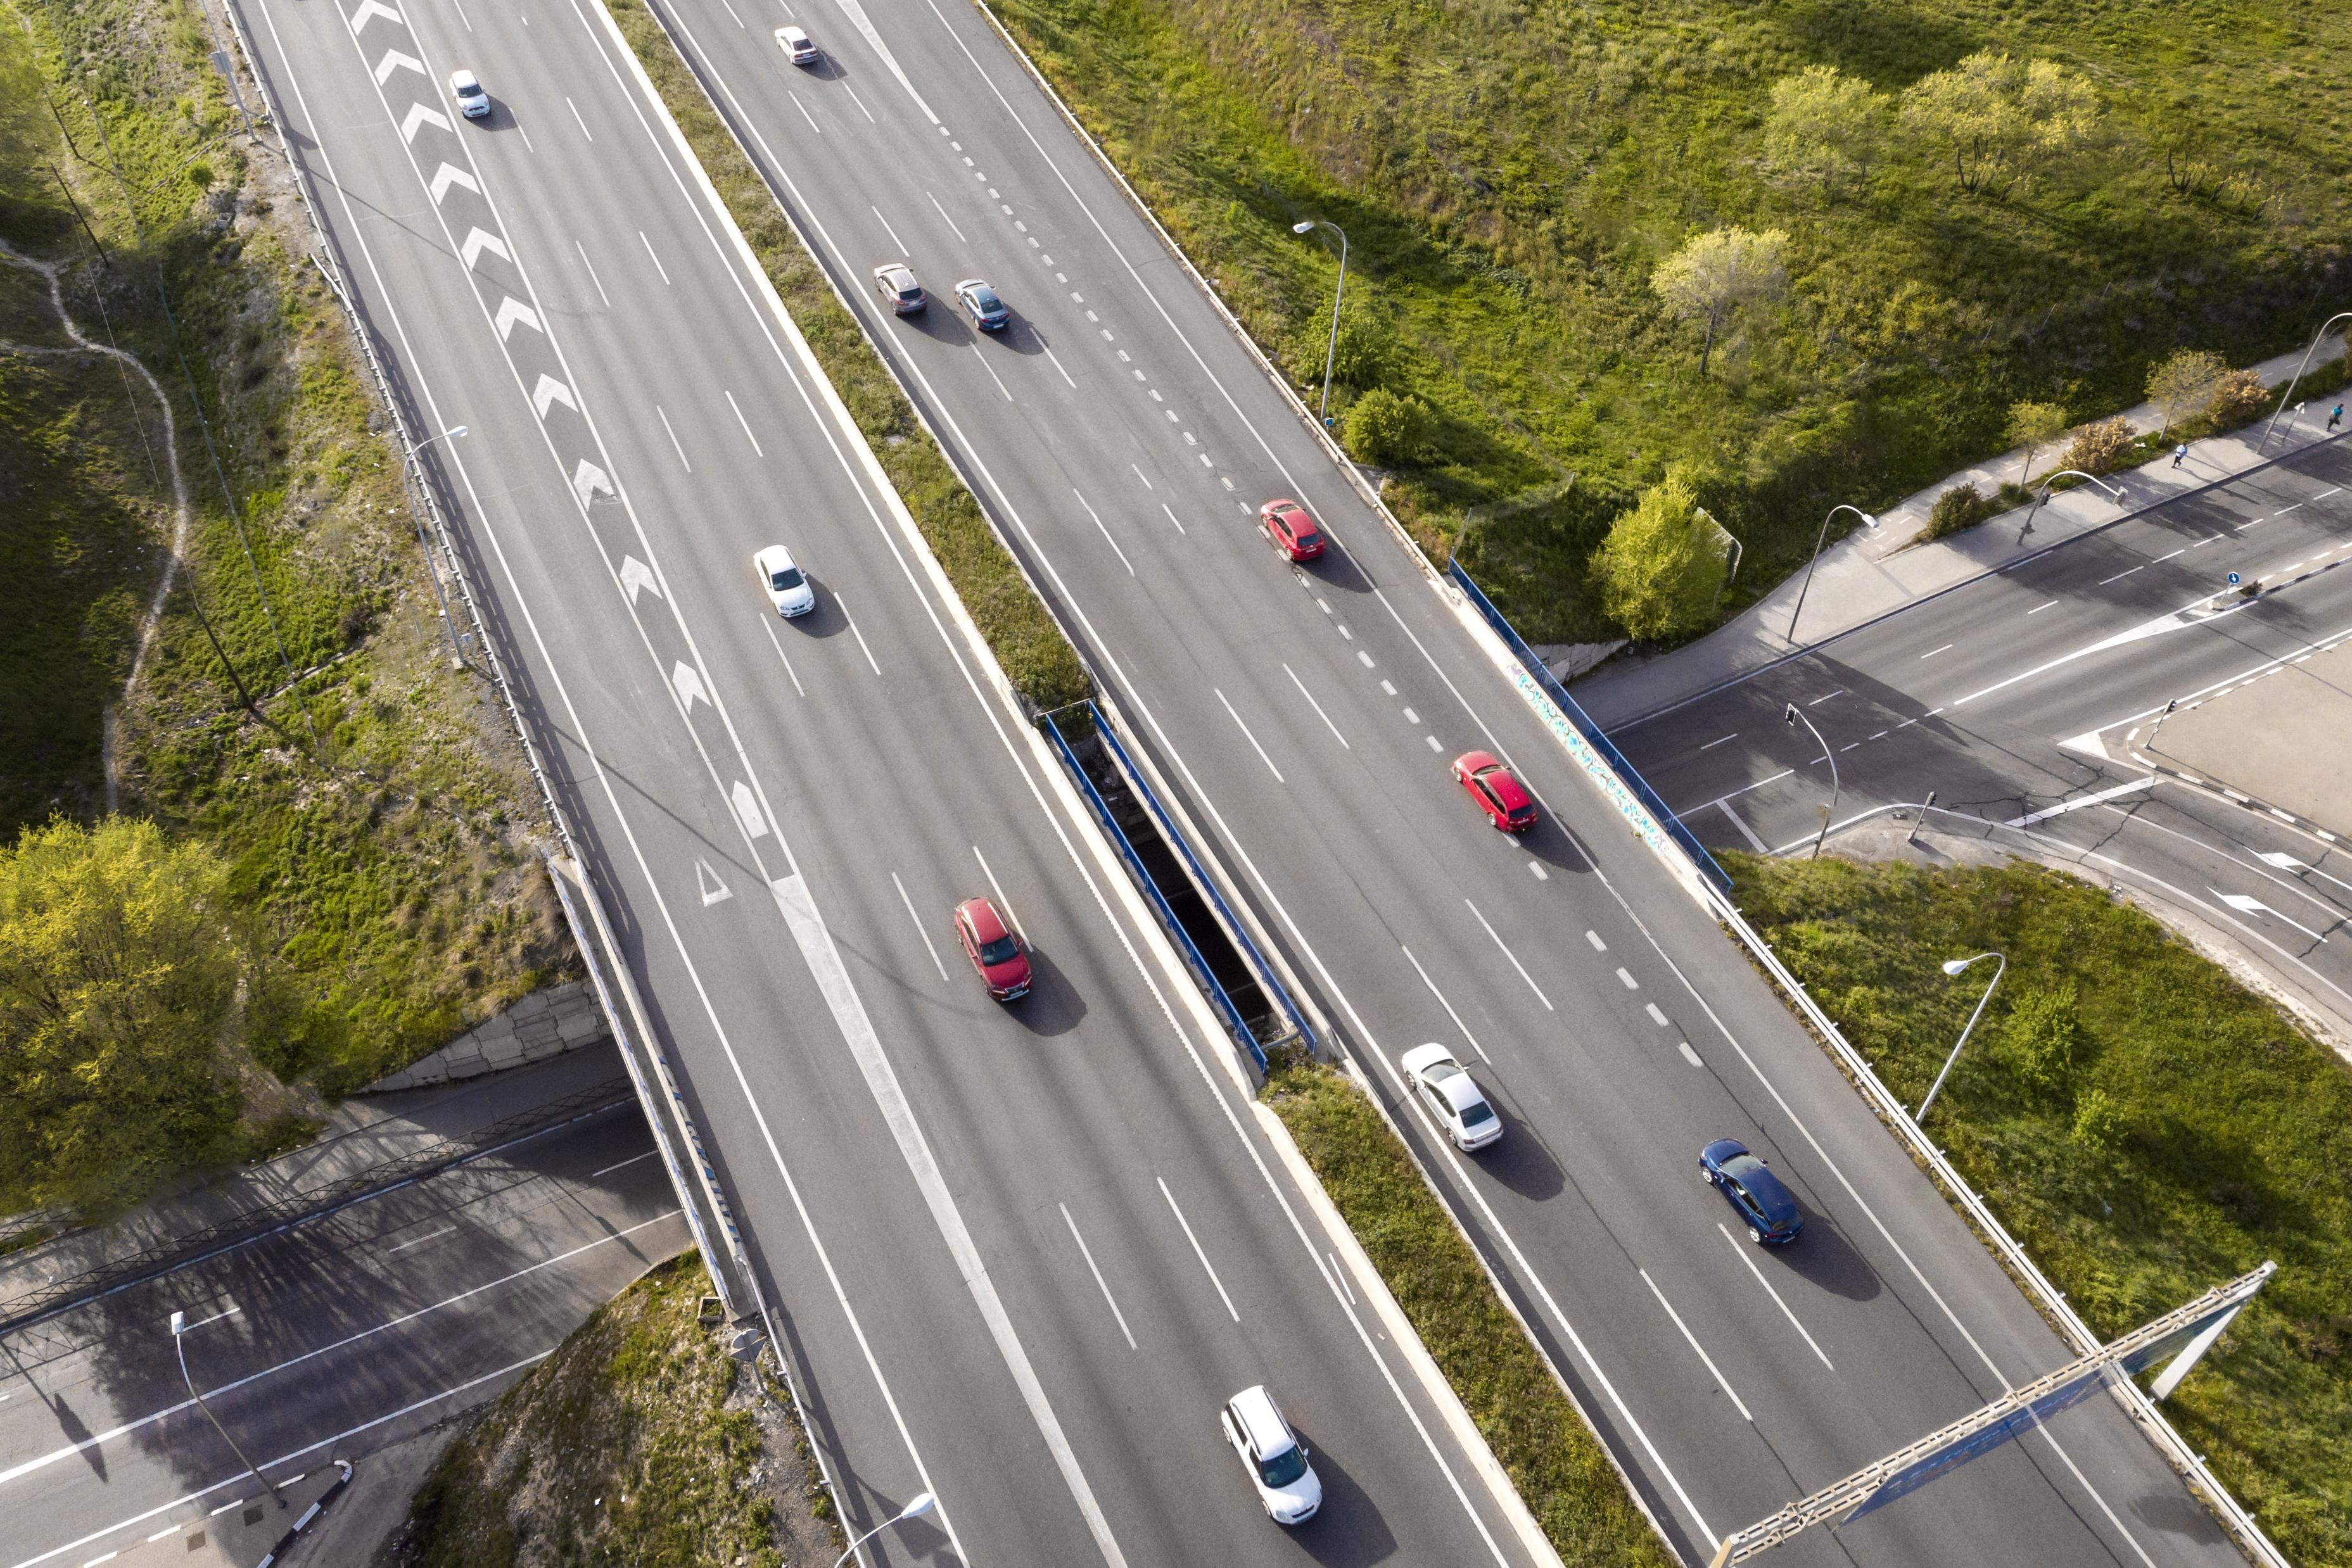
\includegraphics[width=\textwidth]{chapters/Chapitre_3/Figures/autoroute.jpg}
\caption{Highway navigation}
\label{fig:Highway_navigation}
\end{minipage}
\hspace{0.5cm}
\begin{minipage}[b]{0.45\linewidth}
\centering
\includegraphics[width=1.0\textwidth]{chapters/Chapitre_3/Figures/onramp.jpg}
\caption{Highway on-ramp}
\label{fig:on-ramp_highway}
\end{minipage}
\label{fig:scenarios_images}
\end{figure}


In this PhD manuscript, our primary focus lies on exploring the manifold potential of MVS in the context of highway scenarios: 
\begin{itemize} % il faut linker ça avec le speed hamonization

\item \textbf{MVS highway navigation in formation:} Autonomous vehicle formation control, akin to broader concept of highway speed harmonization, exerts an important influence on traffic management, yielding numerous benefits such as heightened road safety, optimized traffic flow, and decreased energy consumption. While human-driven vehicles effortlessly navigate in formation, achieving the same behavior for MVS requires a robust and safe strategy to prevent collisions between the vehicles inside and outside the MVS formation. Additionally, the question of MVS formation stability demands a formal \footnote{Formal: by formal, we refer to the existence of an analytical mathematical model.} systematic response. 



Employing a safe and reliable formation control method allows for reduced inter-vehicle spacing within the MVS paradigm, thus optimizing the road capacity utilization. Since vehicles contend with aerodynamic drag that consumes energy, optimizing inter-vehicle distances can mitigate this drag effort, resulting in energy savings as one of the benefits of MVS navigation in formation (cf. Figure \ref{fig:truck_platooning}) \cite{zhao2021distributed}\cite{Mechnical_simulation}. 

\textbf{\begin{figure}[!h]
        \centering 
        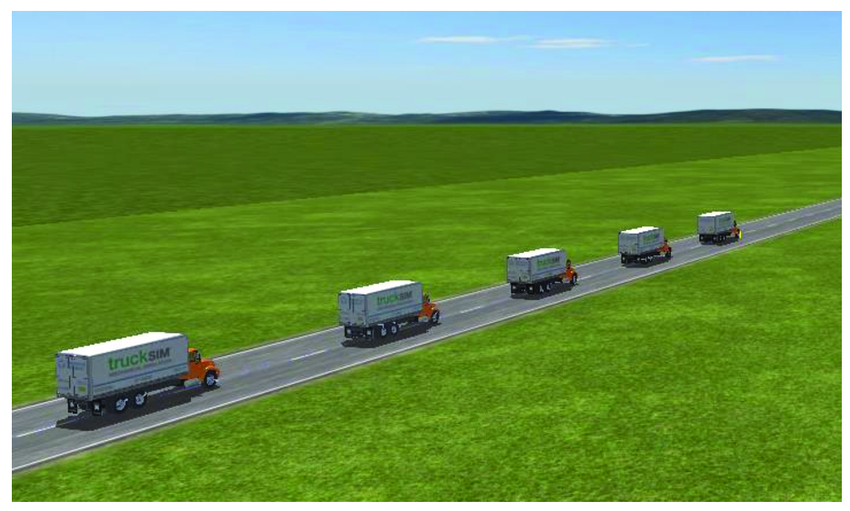
\includegraphics[width=9cm,height=18cm,keepaspectratio]{chapters/Chapitre_3/Figures/Co-simulation-in-Matlab-Simulink-TruckSim.png}
        %\vspace{-2.3mm}
        \caption{Truck platooning \cite{zhao2021distributed}}
        \label{fig:truck_platooning}
        %        \vspace{-5mm}
        \end{figure}}

%\newpage

\item \textbf{Cooperative on-ramp merging on highway:} Traffic merging at highway on-ramps presents significant safety and mobility challenges. The complexity emerges when the vehicle on the on-ramp must make split-second decisions regarding acceleration or deceleration to merge safely into the desired highway lane, often without a clear line of sight (cf. Figure \ref{fig:on_ramp_merging_scenario}). Simultaneously, highway road users must adjust their speeds to accommodate the merging vehicle, potentially disrupting traffic flow and leading to congestion (cf. Figure \ref{fig:on_ramp_merging_scenario}). 


\textbf{\begin{figure}[!h]
        \centering 
        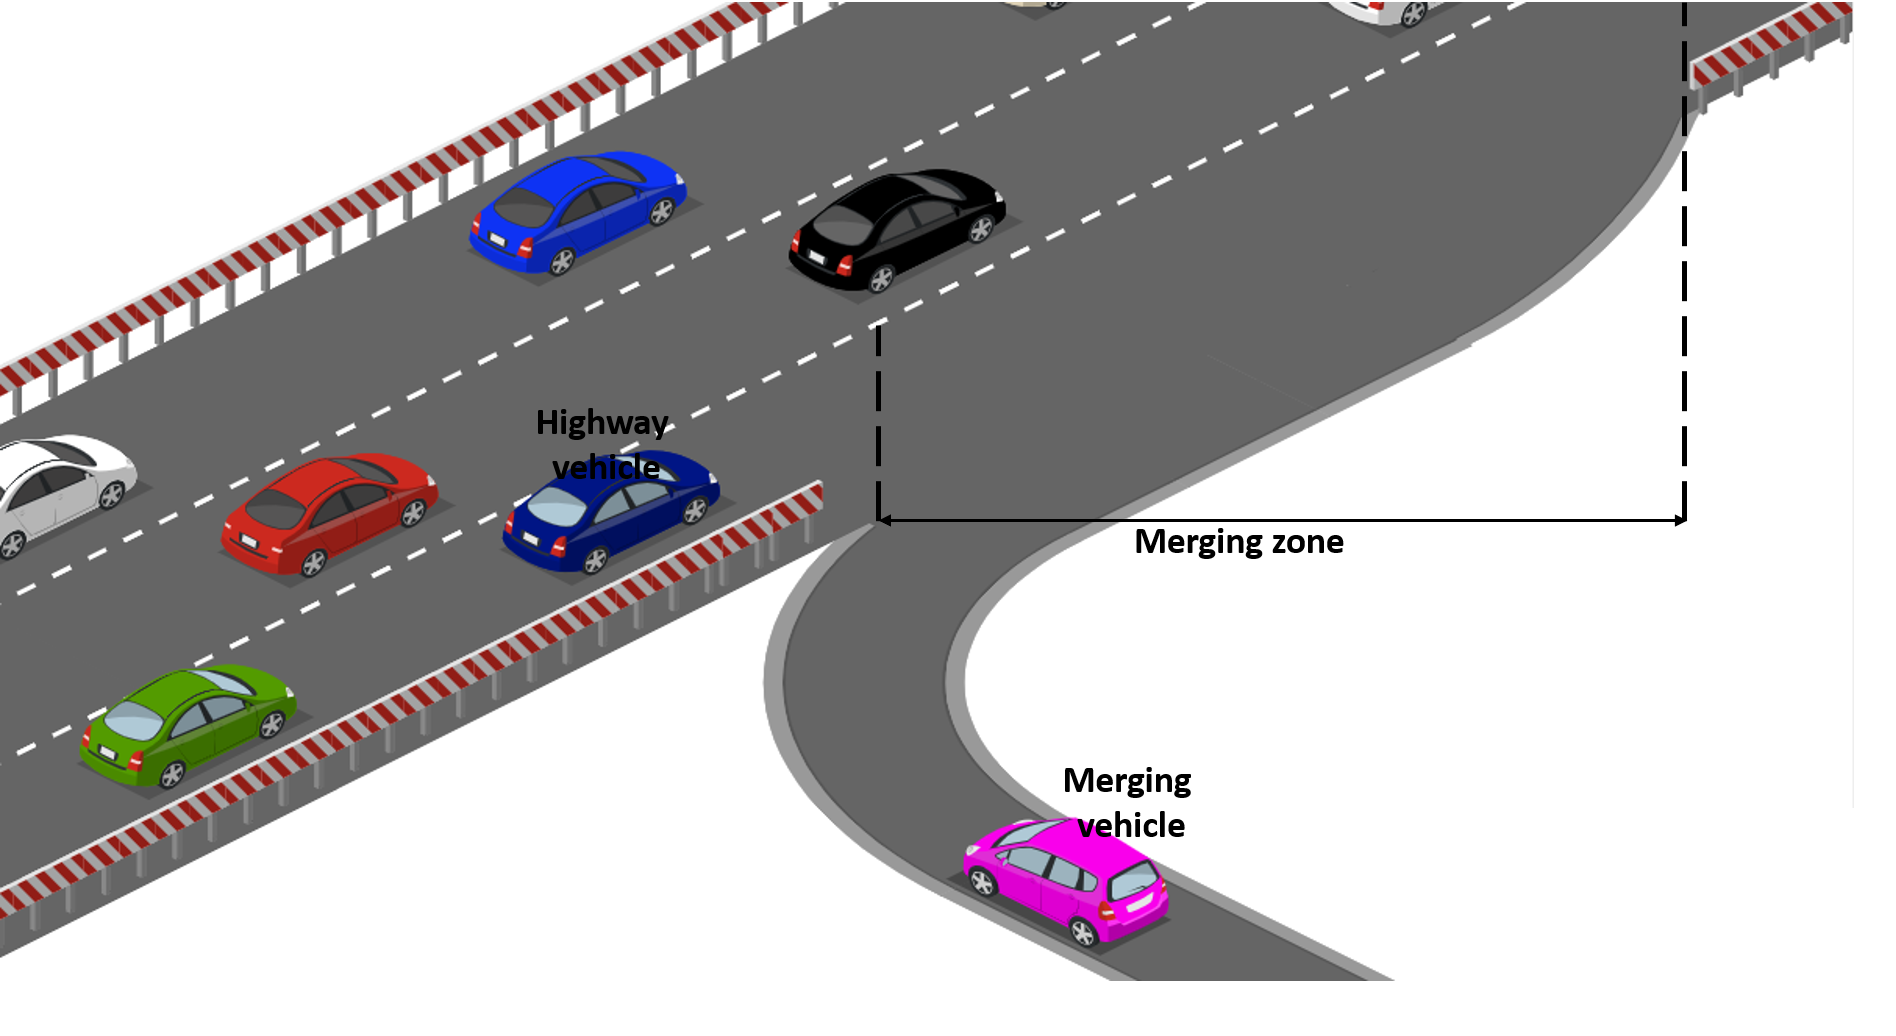
\includegraphics[width=9cm,height=18cm,keepaspectratio]{chapters/Chapitre_3/Figures/CooperativeMerging.png}
       % \vspace{-2.3mm}
        \caption{On-ramp merging on highway}
        \label{fig:on_ramp_merging_scenario}
       %         \vspace{-5mm}
        \end{figure}}









To address these challenges, application of cooperative MVS to highway on-ramp merging scenarios can be explored. Various control architectures can be evaluated to their suitability in managing this specific scenario and its associated complexities \cite{7562449}. 



    
\end{itemize}
    As a result, Section \ref{sec: Highway_cooperative_navigation} shows a comprehensive review of the highway cooperative navigation relative application through the Cooperative Adaptive Cruise Control (CACC) (cf. Section \ref{sec: CACC}).  For the problem of cooperative on-ramp merging on highway, Section \ref{sec: cooperative_merging_on_highway} offers a thorough review of relevant approaches. The MVS reviewed application performance are evaluated through the prism of traffic throughput, energy efficiency, and negotiation. 
    
    
    

   % \textcolor{blue}{Discussion: Je ne sais pas si je peux/dois ajouter notre bibio sur les méthodes en relation avec les cooperative intersection crossing ... L'état de l'art est déjà +/- fait, mais dois-je l'ajouter, sachant que ce chapitre est déjà assez long ? }
    %Further insights into the methods used for cooperative intersection crossing are exposed in Section \textcolor{red}{ajouter la section qui parle des méthodes utilisées pour le intersection crossing }. 



% il faut revoir la décomposition des sections pour donner un plus de sens à cela

\subsection{Highway collaborative navigation} \label{sec: Highway_cooperative_navigation}
Collaborative navigation along a highway entails the intricate task of orchestrating the maneuvers of a fleet of vehicles, collectively referred to as MVS in formation navigation in highway, to function as a cohesive unit known as a formation (cf. Section \ref{sec: formation_control_theory}). Advances in communication technology have ushered in the era of V2V communication (cf. Section \ref{sec: communication}), enabling the exchange of information among vehicles within the same formation. 

Traditionally, vehicles on the road tend to follow each other, creating platoon-based formations (cf. Figure \ref{fig:platoon_formation}). For human-operated vehicles, this platoon behavior is a natural occurrence, easily observable in everyday driving scenarios. However, for MVS, adhering to lanes and maintaining safe distances and velocities when following nearby vehicles become more complex endeavor. This complexity arises primarily from the need to effectively manage the dynamics of MVS vehicles, underscoring the requirement for cooperative control over these dynamics.

\textbf{\begin{figure}[!b]
        \centering 
        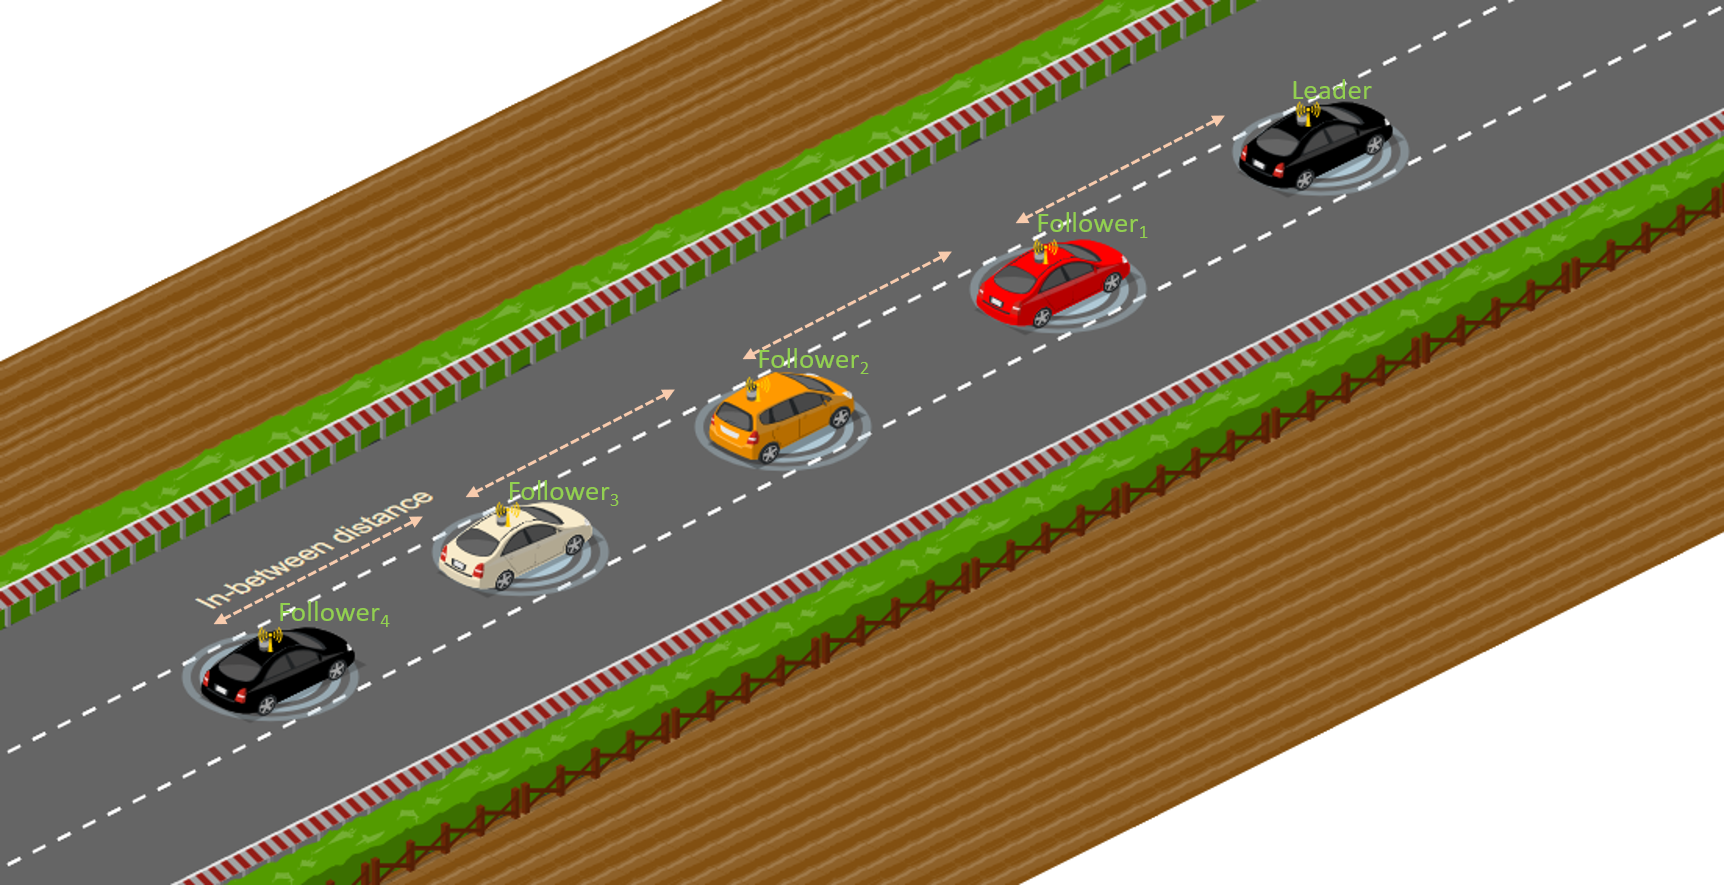
\includegraphics[width=10.5cm,height=18cm,keepaspectratio]{chapters/Chapitre_3/Figures/cooperative_navigation_in_formation_on_highway}
        %\vspace{-2.3mm}
        \caption{Platoon-based navigation in formation on highway}
        \label{fig:platoon_formation}
             %   \vspace{-5mm}
        \end{figure}}


The primary objective of platoon formation control is to ensure that all vehicles within a platoon travel at the same velocity, adhering to the desired one-dimensional spacial configuration, which is stipulated by a predefined inter-vehicle spacing strategy \cite{jia2015survey}. Consequently, the formation of a platoon-based shape necessitates the development of specialized algorithms, controllers and strategies \cite{mariani2021coordination}. 


In the forthcoming section, we will introduce the concept of Cooperative Cruise Control (CACC) as an important module for executing cooperative navigation maneuvers on the highway. It is proposed in what follows to delve into collaborative navigation within formation and explore its ramifications on highway throughput, energy efficiency and its synergy with negotiation. 


\subsubsection{Cooperative Adaptive Cruise Control (CACC)} \label{sec: CACC}
The core of the CACC concept lies on the fusion of Adaptive Cruise Control (ACC), a subset of automated longitudinal speed control systems, with a cooperative module empowered by the V2V communication and/or V2I communication (cf. Section \ref{sec: communication}) \cite{shladover2015cooperative}.

Over the past decade, considerable advancements in MVS technologies have been achieved. MVS now possess the capability not only to autonomously navigate using onboard sensors but also to communicate with other vehicles via V2V communication. The terms of CACC have been used with varying interpretations, leading to different perceptions of their functions and capabilities in the context of CACC and platooning-based solutions. In CACC systems, MVS exchange their parameters via the V2V communication without a central management unit \cite{wischhof2005information}. Consequently, CACC leverages V2V communication (cf. Figure \ref{fig:platoon_formation}) to enable the vehicles part of the MVS to form platoons and travel at synchronized speed \cite{wang2019survey}. This synchronization is achieved by minimizing the error $d_e$ between the desired distance $d_d$ (depending on the spacing policy and the current dynamic of the MVS) and the current inter-vehicle distance $d_{(.)→(.)}$ (cf. Figure \ref{fig:CACC}). 

        \begin{figure}[h!]
        \centering 
        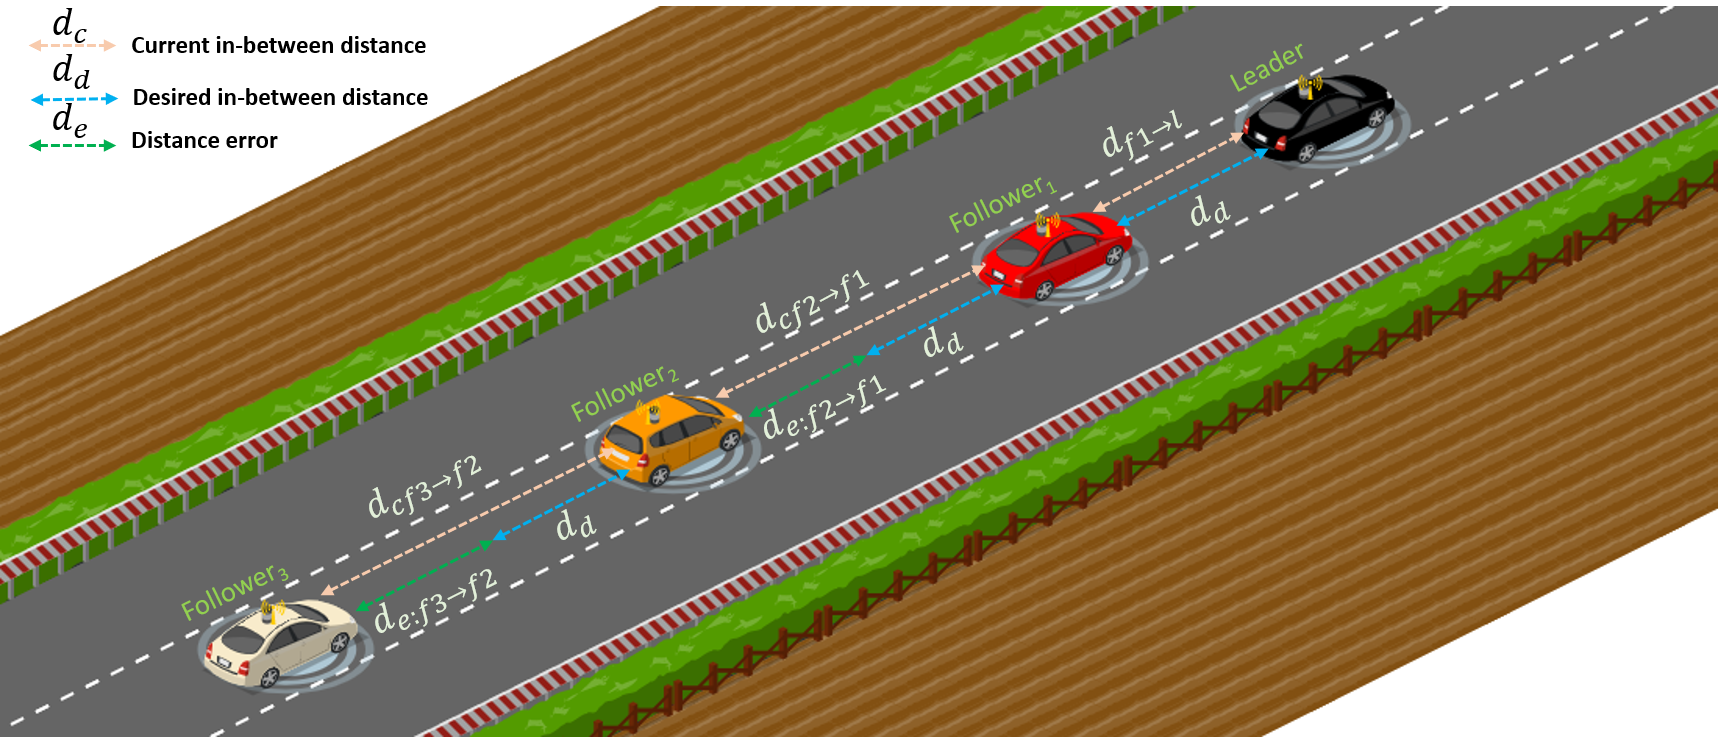
\includegraphics[width=11cm,height=18cm,keepaspectratio]{chapters/Chapitre_3/Figures/cooperative_adaptive_cruise_control}
       % \vspace{-2.3mm}
        \caption{Cooperative Adaptive Cruise Control}
        \label{fig:CACC}
                %\vspace{-5mm}
        \end{figure}



Through the sharing of vehicle information, including acceleration, speed, and position, MVS with a certain communication range of the roadside unit collaborate to obtain several benefits: 

\begin{itemize}
    \item Enhanced driving safety is achieved through reduced actuation times compared to manual driving, along with improved anticipation of the future actions of the MVS. 

    \item Increased highway capacity results from reduced time/distance headway between the MVS. 

    \item Reduced energy consumption and pollutant emissions stem from minimized unnecessary velocity changes and decreased aerodynamic drag on following vehicles. 
\end{itemize}


        
The vehicle control strategy plays also a role in CACC systems as it determines the vehicle's dynamics. Specifically, the longitudinal control strategy has been extensively studied, \cite{wang2018review}\cite{dey2015review}\cite{nowakowski2010cooperative}, as vehicles operating in CACC mode must maintain the same longitudinal speed as other vehicles in the platoon while sustaining a constant longitudinal distance/headway relative to their preceding vehicle. Various longitudinal controllers have been proposed to address different objectives, such as platoon formation, optimizing fuel consumption, or ensuring system stability \cite{moser2017flexible}\cite{nie2020adaptive}. 

The literature related to the CACC includes several coordination approaches (e.g., consensus-based, optimization-based, etc.). A comprehensive review of these approaches can be found in \cite{wang2018review}\cite{dey2015review}\cite{liu2023systematic}.


One of the objective of this PhD work is take advantage of the MVS advantages (e.g. safety, passenger comfort, energy efficiency). From this perspective, the optimization techniques are well-suited to include these several criteria.  The following sections will undertake an in-depth analysis of various longitudinal controllers founded, based on optimization techniques.


\paragraph{Optimal Control} \label{sec: optimal-control} 
%In addition of MPC, other optimal control methodologies have been explored in the context of CACC. 

Optimal control has been employed to optimize energy consumption or travel time in \cite{massera2017safe}. While many consensus-based control approaches (cf. Section \ref{sec:consensus_control}) focus solely on vehicle speed and position, simplifying the longitudinal control to a single or double integrator model under the assumption of linearity, optimal control techniques often consider non-linearity and constraints \cite{wang2018review}\cite{dey2015review}\cite{shao2017robust}. These constraints may involve vehicle power-train dynamics and aerodynamics \cite{turri2018fuel}. 

In numerous cases where optimal control is applied to CACC systems, the objective function minimizes the total energy consumed by the vehicle traveling within a designated area. For instance, in the Eco-CACC system proposed in\cite{yang2016eco}, it computes the fuel-optimum vehicle trajectory through a signalized intersection, the optimal control problem is defined as: 


\begin{equation}
\min_{a_{-}, a_{+}} \int_{t_{0}}^{t_{0}+T} F(v(t), v'(t)) dt
\end{equation}

subject to

\begin{equation}
\int_{t_{0}}^{t_{0}+T} v(t) dt = d + l
\end{equation}

\begin{equation}
0 \leq a_{-} \leq a_{-}^{s}
\end{equation}

\begin{equation}
0 \leq a_{+} \leq a_{+}^{s}
\end{equation}

Here, $F(\cdot, \cdot)$ represents a nonlinear function of speed $v(t)$ and acceleration $v'(t)$, estimating the energy consumption rate based on vehicular speed and acceleration levels. $a_-$ and $a_+$ are the upstream deceleration and the downstream acceleration levels, respectively. $d$ and $l$ are the length of the control zone before and in the signalized intersection, respectively. 







\paragraph{String stability} \label{sec: string_stability}

String stability is a fundamental requirement to ensure the safety of the CACC system. It aims to attenuate distance error, velocity, or acceleration along the upstream direction in a platoon, as discussed in \cite{rajamani2011vehicle}. The problem of string stability can be formulated as: 

\begin{equation}
|y|{_\infty} \leq|u|{_\infty}
\end{equation}

Here, $y$ represents the scalar output of distance error, velocity, or acceleration of the following vehicle $i+1$, and $u$ represents the scalar output of distance error, velocity, or acceleration of the preceding vehicle $i$. String stability is guaranteed if:

\begin{equation}
\left|\frac{Y(s)}{U(s)}\right|_{\infty} \leq 1
\end{equation}

\noindent where $Y(s)$ and $U(s)$ are the Laplace transforms of $y$ and $u$, respectively.

Numerous works have analyzed the string stability of CACC systems \cite{wang2018review}\cite{nowakowski2010cooperative} \cite{9310215}, and some conclusions have been proposed to ensure string stability: 

\begin{itemize}
    \item If a constant distance spacing policy is adopted for vehicle spacing, the predecessor-follower (cf. Section \ref{sec: communication}) information flow may not guarantee string stability. Extending the information by broadcasting the leader's information to the following vehicles, using a predecessor-follower-leader information flow (cf. Section \ref{sec: communication}), for example, can ensure string stability. 

    \item To relax the formation rigidity imposed by the constant spacing policy, a constant time headway spacing policy can be employed, ensuring string stability by allowing the inter-vehicle distance to depend on the vehicle's velocity \cite{wang2018review}. 
\end{itemize}


\paragraph{Model Predictive Control (MPC): } \label{MPC}
Traditionally, Model Predictive Control (MPC) is framed within the state space framework for single vehicle, where controlled system is described by a linear model as expressed in \cite{stanger2013model}: 
\begin{equation}
\dot{x}(t) = Ax(t) + Bu(t), \quad x(0) = x_{0}
\end{equation}

Here, $x(k) \in \mathbb{R}^n$ represents the state input, and $u(k)\in \mathbb{R}^p$ represents the control input. With $n$ and $p$ are the the state variables and inputs numbers respectively. $A$ is the state matrix, with $dim [A]=n\times n$, and $B$ is the input matrix, with $dim [B]=n\times p$. $x_0$ is the initial state vector. Typically, a receding horizon implementation is formulated as an optimization problem, such as:

\begin{equation}
J_{u(t)}(x_{0}) = \min_{a(t)} \int_{0}^{T} [q_{f}(v(t), a(t)) + \gamma] dt
\end{equation}

Subject to:

\begin{equation}
\Delta \dot{x}(t) = v_{p}(t) - v(t)
\end{equation}

\begin{equation}
\dot{v}(t) = a(t)
\end{equation}

\begin{equation}
\Delta x(t) \geq \Delta x_{\min , 0}+h_{\min } v(t)
\end{equation}

\begin{equation}
\Delta x(t) \leq \Delta x_{\max , 0}+h_{\max } v(t)+\gamma r
\end{equation}

\begin{equation}
a_{\min} \leq a(t) \leq a_{\max }(v(t))
\end{equation}

\begin{equation}
v_{\min} \leq v \leq v_{\max }
\end{equation}

In this context, $q_f$ represents the current fuel consumption depending on $v(t)$ and $a(t)$, where $v(t)$ is the ego-vehicle's velocity and $a(t)$ is its acceleration. $v_{p}(t)$ represents the preceding vehicle's velocity. $\Delta x(t)$ denotes the actual inter-vehicle distance, with $\Delta x_{\min , 0}$ and $\Delta x_{\max , 0}$ being the minimum and maximum distances when stationary. $h_{\min }$ and $h_{\max }$ correspond to the minimum and maximum time headway, associated with the minimum and maximum inter-vehicle distances. The relaxation aspect is introduced through the slack variable $\gamma$ and relaxation parameter $r$. Constraints are also applied to acceleration ($a_{min}$ and $a_{max}$) and velocity ($v_{min}$ and $v_{max}$).


Typically, centralized MPC systems assume knowledge of all the states for computing control inputs. However, in practical applications, especially in dynamic scenarios like highway traffic, gathering information from all the vehicles to compute a large-scale optimization problem is not always feasible. This limitation has led to the development of Distributed Model Predictive Control (DMPC) \cite{caruntu2016distributed}\cite{negenborn2014distributed}, and stochastic MPC (SMPC) to include the uncertainty of the system \cite{moser2015cooperative}.





\subsubsection{Evaluation of the highway collaborative navigation approaches}
As discussed in Section \ref{sec: CooperativeNavigation-Scenarios Overview}, MVS collaborative navigation is linked with several advantages. In this section, an extensive examination of MVS formation navigation in highway is presented, with a focus on aspects such as traffic throughput, energy efficiency, and negotiation.

\paragraph{Traffic throughput} \label{sec: highway_Traffic_throughput}

The primary goal of the CACC systems is to establish and regulate platoon-based formations. Consequently, the advantages of CACC systems can be considered as benefits for formation-based navigation on highways. 

The impact of platoon enabled by CACC on highway throughput was investigated in \cite{van2006impact}. In this research, a stochastic microscopic-traffic simulation model was developed to assess various of traffic flow performance, including safety, exhaust-gas emissions, and noise emissions. The proposed model utilizes real traffic measurements, such as instances, lanes speeds, and vehicle lengths, to generate traffic scenarios at the beginning of simulations runs. The simulations demonstrated that the presence of more CACC-equipped vehicles in traffic leads to higher average velocities. Regarding traffic throughput, scenarios with 100 \% CACC-equipped vehicles showed the best performance compared to other mixing penetration scenarios. 

In \cite{liu2018modeling}, a CACC modeling framework was proposed, incorporating interactions between CACC-equipped vehicles and manually driven vehicles in mixed traffic. This framework included lane-changing rules and automated speed control to ensure realistic CACC performance. Several simulations were conducted on a 4-lanes freeway segment with an on-ramp and off-ramp lanes. The case study compared basic CACC-operated vehicles with Multi-Lanes CACC (ML-CACC)-operated vehicles for different market penetrations. Results indicated that traffic flows with CACC market were consistently lower that those with ML-CACC. 

The study in \cite{jin2020analysis} shows the effect of platooning on mixed traffic and its impact on improving highway throughput. To address this scenario, a new fluid model of mixed-autonomy traffic flow was introduced, which was then used to analyze and design platoon coordination strategies. Simulations were conducted to study the effect of platoon penetration on highway throughput. The results showed that traffic throughput increased with higher platoon fractions on the highway. The study also explored the impact of platoon size, revealing the presence of an optimal platoon size. 


\paragraph{Energy efficiency} \label{sec: energy_efficiency}
Vehicle platooning offers a significant opportunity to enhance energy efficiency by substantially reducing the distance between vehicles, thereby decreasing the aerodynamic drag coefficient \cite{wadud2016help}. The extent of drag reduction in platooning depends on factors such as the vehicle shapes with the platoon, their arrangement, and the distance between them. Savings are most pronounced for vehicles positioned in the middle of the platoon, and the overall savings increase with the number of vehicles in the platoon. For instance, when two vehicles maintain 1-meter gap between them, the average gap reduction is estimated to be around 10 \% \cite{zhu2011simulation}. In cases where the platoon consists of a mix of vehicle types, drag reduction has been estimated at 20\% \cite{schito2012numerical}, and even up to 40 \% \cite{duan2007effects}. In scenarios involving long platoons of vans (five or more vehicles) spaced 0.5 to 1-meters apart, drag reduction of up to 44 \% to 55\% has been reported in \cite{schito2012numerical}. 

Platoon-based formations facilitated by CACC systems also lead to energy efficiency improvements by minimizing unnecessary changes in velocity. In \cite{wang2017developing}, an approach was proposed to minimize energy consumption and pollutant emissions within platoons during various stages, including sequence determination, gap closing and opening, platoon cruising with gap regulation, and platoon joining and splitting. Compared to consensus-based (cf. Section \ref{sec:consensus_control}) CACC system, the results demonstrated that an ECO-CACC (cf. Section \ref{sec: CACC}) could reduce global energy consumption by 1.5 \% during platoon formation and 2 \% during platoon reconfiguration phases \cite{wang2017developing}.

In \cite{bichiou2020vehicle}, an energy consumption model was developed for various types of vehicles, including internal combustion light-duty vehicles, electric vehicles, hybrid electric vehicles, buses and trucks. This model aimed to quantify the effects of platooning on fleet fuel consumption. The findings indicated that energy consumption reductions of up to 3\%, 3.5\%, 4.5\%, 10\%, and 15\%, respectively. 

It becomes evident that vehicles platooning is especially well-suited for heavy-duty vehicles, particularly on highways where travel is at high speeds, leading to substantial aerodynamic drag. Trucks, which often cover long distances on highways, can benefits from joining neighboring trucks to form platoons, even if they have different starting points and destinations. For an in-depth analysis of fuel economy in truck platooning, refer to \cite{zhang2020fuel}. %\textcolor{red}{ajouter des reference sur le truck platooning, ajouter les travaux du gars qui est venus présenter ses travaux au bureau sur platooning}. 

\paragraph{Negotiation} \label{sec: Negotiation_platoon}

To date, the literature lacks of substantial exploration of negotiation- and agreement-based approaches concerning navigation in formation, applied to the case of highways and MVS formation reconfiguration in highway (cf. Figure \ref{fig:negotiation_CACC}) \cite{mariani2021coordination}. This absence may stem from several factors, including unsuitability of such approaches or simply insufficient exploration of these possibilities. One key reason for scarcity of negotiation in this context could be the limited scope for negotiation or discussion with a platoon during cruising. For instance, while one might argue that leader selection could be a negotiation topic, leaders are typically chosen strategically and functionally, often as the vehicle positioned at the front of the formation. Similarly, negotiation speed profiles may not be a significant consideration since the primary goal of a platoon is to travel safely at the maximum allowable speed \cite{mariani2021coordination}. 
\textbf{\begin{figure}[!h]
        \centering 
        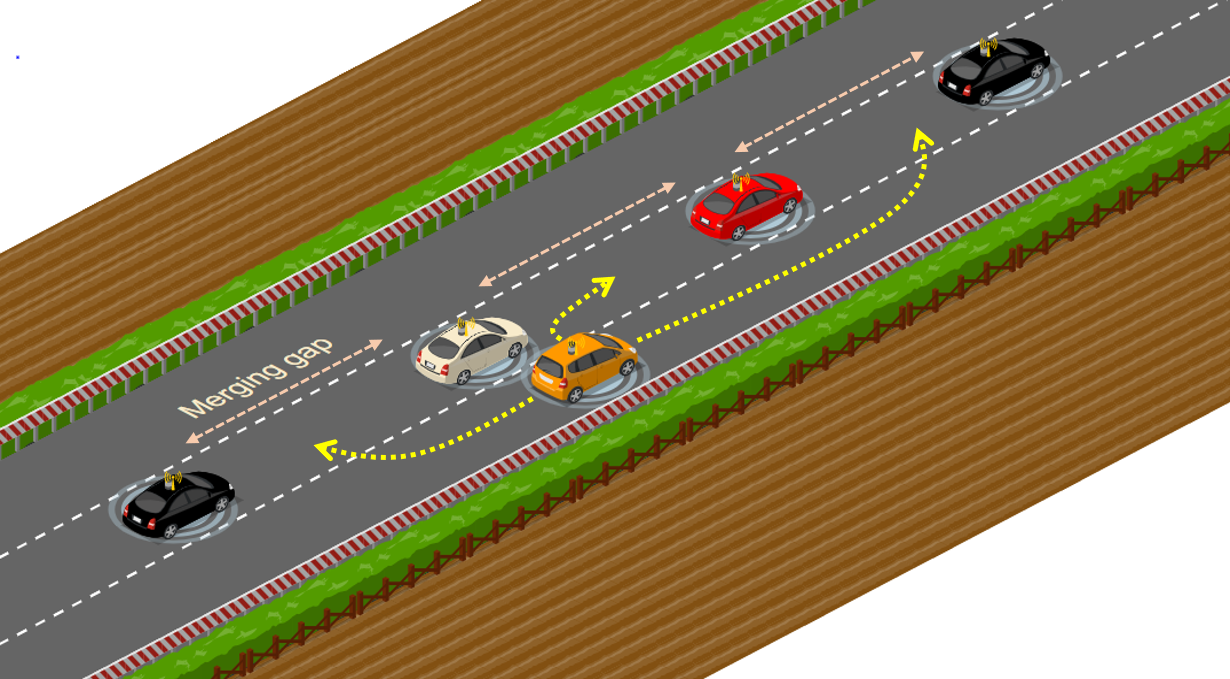
\includegraphics[width=11cm,height=18cm,keepaspectratio]{chapters/Chapitre_3/Figures/cooperative_merging_on_highway}
       % \vspace{-2.3mm}
        \caption{Negotiation-based merging in highway}
        \label{fig:negotiation_CACC}
          %      \vspace{-5mm}
        \end{figure}}


However, a potential avenue for exploration is negotiation platoon reconfiguration. Platoon-based formations operate with dynamic environments, such as highways, and are subject to various maneuvers, including vehicles joining, splitting, or changing lanes (individually or as a formation). These maneuvers need to be executed with a global perspective to ensure safety and efficiency, while also being fair in terms of the efforts required from each vehicle. For instance, consider the splitting maneuver depicted in Figure \ref{fig:negotiation_CACC}. Platoon members could engage in discussions where each vehicle proposes its solution to create the desired gap. A negotiation mechanism could then be employed to select the best proposition, taking into account safety and efficiency. 

In practice, scenarios like these are often managed by the platoon leader \cite{amoozadeh2015platoon}. In this work, the authors introduced a platoon management protocol supporting three fundamental maneuvers: merging, splitting, and lane changes. The reconfiguration protocol relies on centralized platoon coordination, where all maneuvers are decided and planned by the platoon leader, and followers follow orders and send requests to and from the leader. However, this approach has limitations associated with centralization (cf. Section \ref{sec:CentralizedArchitecture}), such as restricted flexibility (i.e., typically limited to the communication range) and a lack of formal methods for analyzing the stability of the proposed solutions. 


In addition to the above cooperative highway navigation approaches, on-ramp merging on highway is also one scenario subject to MVS cooperative navigation. The following section presents an overview of the approaches related to MVS on-ramp merging on highway.  
 
\subsection{Collaborative on-ramp merging on highway} \label{sec: cooperative_merging_on_highway}
The merging of traffic at highway on-ramp presents a significant challenge, leading to safety and traffic flow concerns. This challenge becomes particularly pronounced for the merging vehicles, as they must make real-time decisions regarding acceleration or deceleration to safely integrate into the mainlines traffic, often without a clear line of sight. Simultaneously, the drivers on the highway may need to adjust their speeds to facilitate the smooth entry of merging vehicles, potentially, disrupting traffic flow and can induce congestion. In response to these complex issues, researchers have explored the concept of cooperative merging, specifically involving MVS, to address the merging problem at highway on-ramp. 

One can note that the corner stone idea behind collaborative on-ramp merging on highway is to minimize the global effort provided by each vehicle while performing the merging scenario. Naturally, the idea of Prioritizing the stability of the already established vehicle groups (platoons) arises as an evidence. The works in \cite{SCHOLTE2022103511}\cite{s23094401}\cite{9781345} propose several strategies for vehicle merging in an already established platoon with low collaborative efforts.

Various control algorithms have been proposed and implemented to enable the vehicles part of the MVS to merge with one another in a cooperative manner. An extensive review of existing research can be found in \cite{7562449}\cite{awal2013optimal}\cite{zhu2022merging}\cite{bevly2016lane}. In this section, it is proposed to evaluate the existing literature related to cooperative on-ramp merging on-highway through the prism of traffic throughput (cf. Section \ref{sec: on-ramp_traffic_throughput}), energy efficiency (cf. Section \ref{sec: merging_energy_efficiency}), and its implication with negotiation (cf. Section \ref{sec: merging_negotiation}). 

\subsubsection{Traffic throughput} \label{sec: on-ramp_traffic_throughput}
Enhancing highway traffic flow throughput seamless merging at highway on ramps has been a widely explored challenge in the literature. Initially, centralized approaches (cf. Figure \ref{fig:Centralized_merging}) were introduced, utilizing a merging coordinator with support of V2I communication. For instance, in \cite{4047597}, a two-layer centralized controller was proposed based on heuristic rules derived from empirical observations of system behavior. The first layer established the merging sequence by estimating each vehicle's merging time, assuming constant-speed travel. The second layer determined the necessary constant acceleration to resolve conflicts identified during the merging sequence. However, heuristic-based approaches are limited in their adaptability to dynamic environments, and their optimality is not rigorously proven due to the absence of formal optimization algorithms approach. 

\textbf{\begin{figure}[!t]
        \centering 
        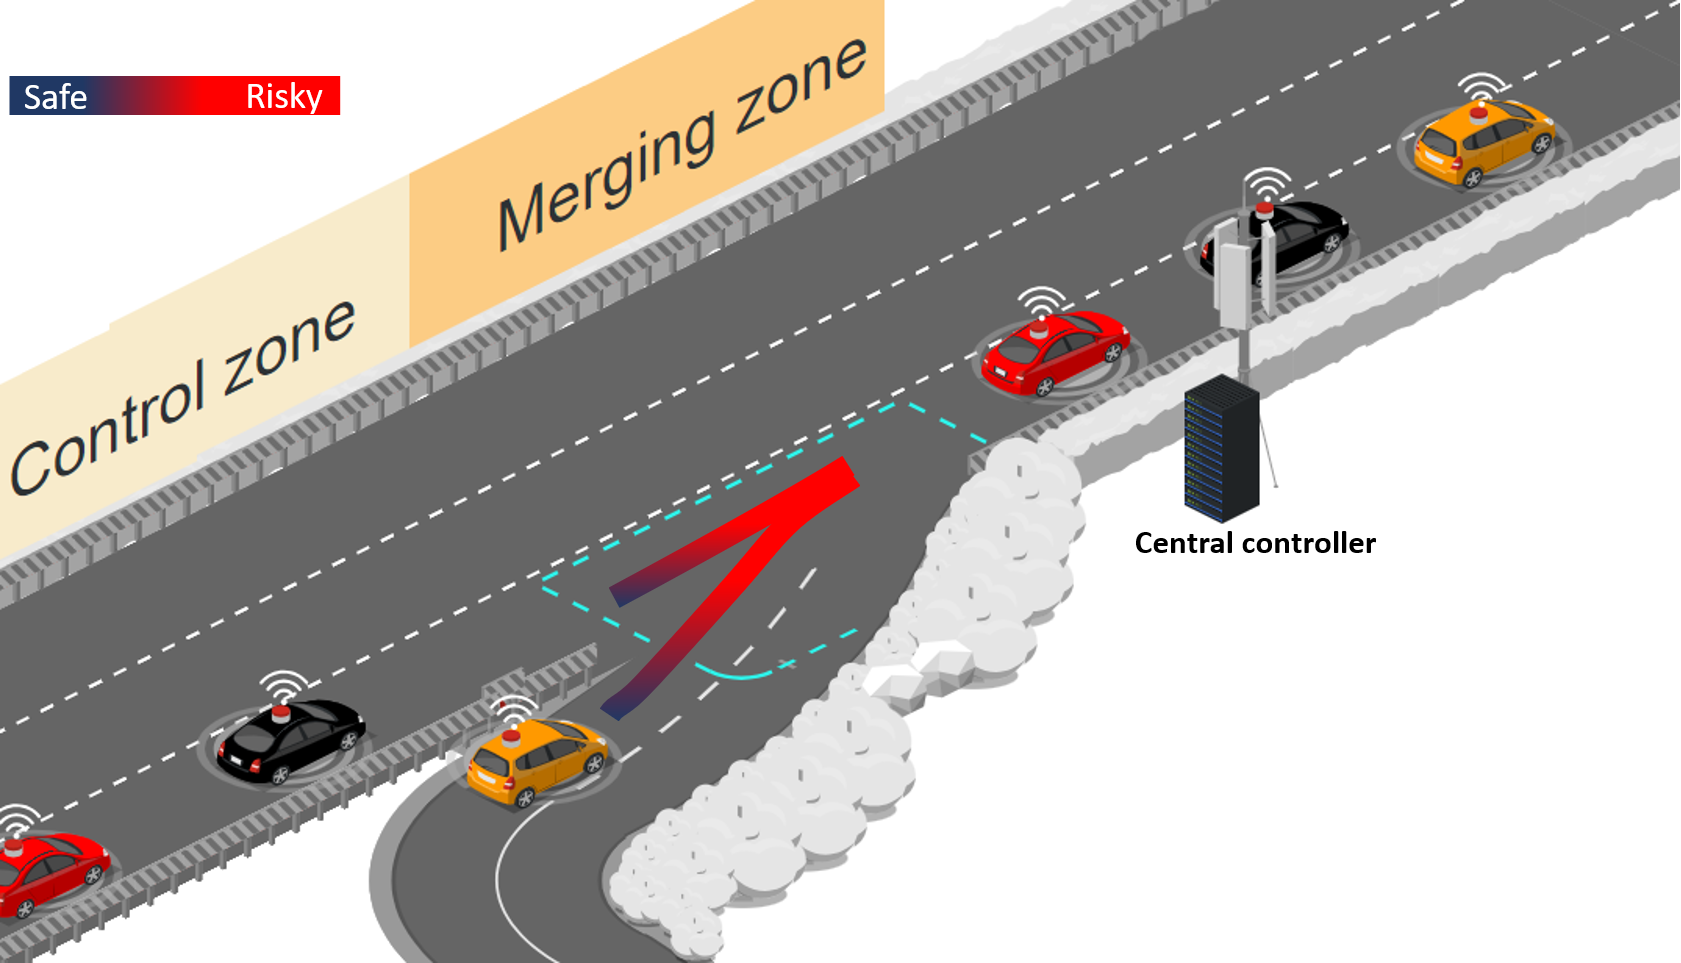
\includegraphics[width=10.5cm,height=18cm,keepaspectratio]{chapters/Chapitre_3/Figures/Centralized_cooperative_on_ramp_merging.png}
        %\vspace{-2.3mm}
        \caption{Centralized collaborative on-ramp merging on highway}
        \label{fig:Centralized_merging}
                %\vspace{-5mm}
        \end{figure}}

 %\newpage
To address the optimality concerns in passing sequences, several centralized methods have been developed in the literature, focusing on optimizing travel time to increase highway throughput. These methods use the communication coordinator's responsibility to optimize the passing sequence order based on merging times. An example of optimizing problem formulation is developed below \cite{7562449}, the particularity of this approach resides on reliance on the merging zone crossing time, what makes it less road geometry dependent and more generic: 

\begin{equation}
\min_{u} \frac{1}{2} \sum_{j=1}^{m} \sum_{i=1}^{n}\left[t_{j, i}^{\text {out }}-t_{j, i}^{\text {in }}\right]^{2}
\end{equation}

Subject to: 

\begin{equation}
    \begin{aligned}
\dot{x}_{j, i} &=v_{j, i} \\
\end{aligned}
\end{equation}
\begin{equation}
\begin{aligned}
\dot{v}_{j, i} &=u_{j, i} \\
\end{aligned}
\end{equation}
\begin{equation}
\begin{aligned}
t_{j, i}^{\text {out }}-t_{j, i}^{\text {in }} & \geq \Delta T_{a} \\
\end{aligned}
\end{equation}
\begin{equation}
\begin{aligned}
o<v_{j, i}(t, u) & \leq v^{\max } \\
\end{aligned}
\end{equation}
\begin{equation}
\begin{aligned}
x_{j, i}(t) & \leq x_{j, i+1}(t)+\delta \quad \forall t \\
\end{aligned}
\end{equation}
\begin{equation}
\begin{aligned}
x_{j, i}(t) & \leq x_{p, q}(t)+S \quad \forall t, j \neq p, i \neq q
\end{aligned}
\end{equation}


\noindent where $t_{j, i}^{\text {in }}$ and $t_{j, i}^{\text {out }}$ are the times that the vehicle $i$, on the road $j$, enters and exits the merging zone, $\Delta T_{a}$ is the minimum allowed time to cross the intersection at the maximum speed $v^{\max}$, and $\delta$ is the desired safe distance between vehicles on the same road. $S$ is the length of the shared zone.

Another approach, as presented in \cite{7562449}, offered an optimization framework with an analytical closed-form solution for online vehicle coordination at merging zones. Simulations demonstrated significant reductions in travel times and improvements in traffic flow. In addition, in \cite{chou2016coordinated}, the authors introduced an approach that virtually positioned vehicles onto highway's main lane before actual merging, ensuring smooth and safe merging maneuvers. The results indicated substantial improvements in traffic flow when a high percentage of MVS vehicles were involved. 

\paragraph*{Discussion}
While centralized methods have shown promise in addressing highway on-ramp merging, they come with certain limitations. These approaches heavily rely on communication, exacerbating any communication-related issues that may arise. Moreover, their critical flaw lies in fault tolerance; if the central coordinator fails, the entire system may fail. 

To mitigate these issues, decentralized approaches (cf. Figure \ref{fig:Decentralized_merging}) can be considered. These approaches draw inspiration from centralized methods, such as the concept of virtual vehicles/platooning. 

\textbf{\begin{figure}[!h]
        \centering 
        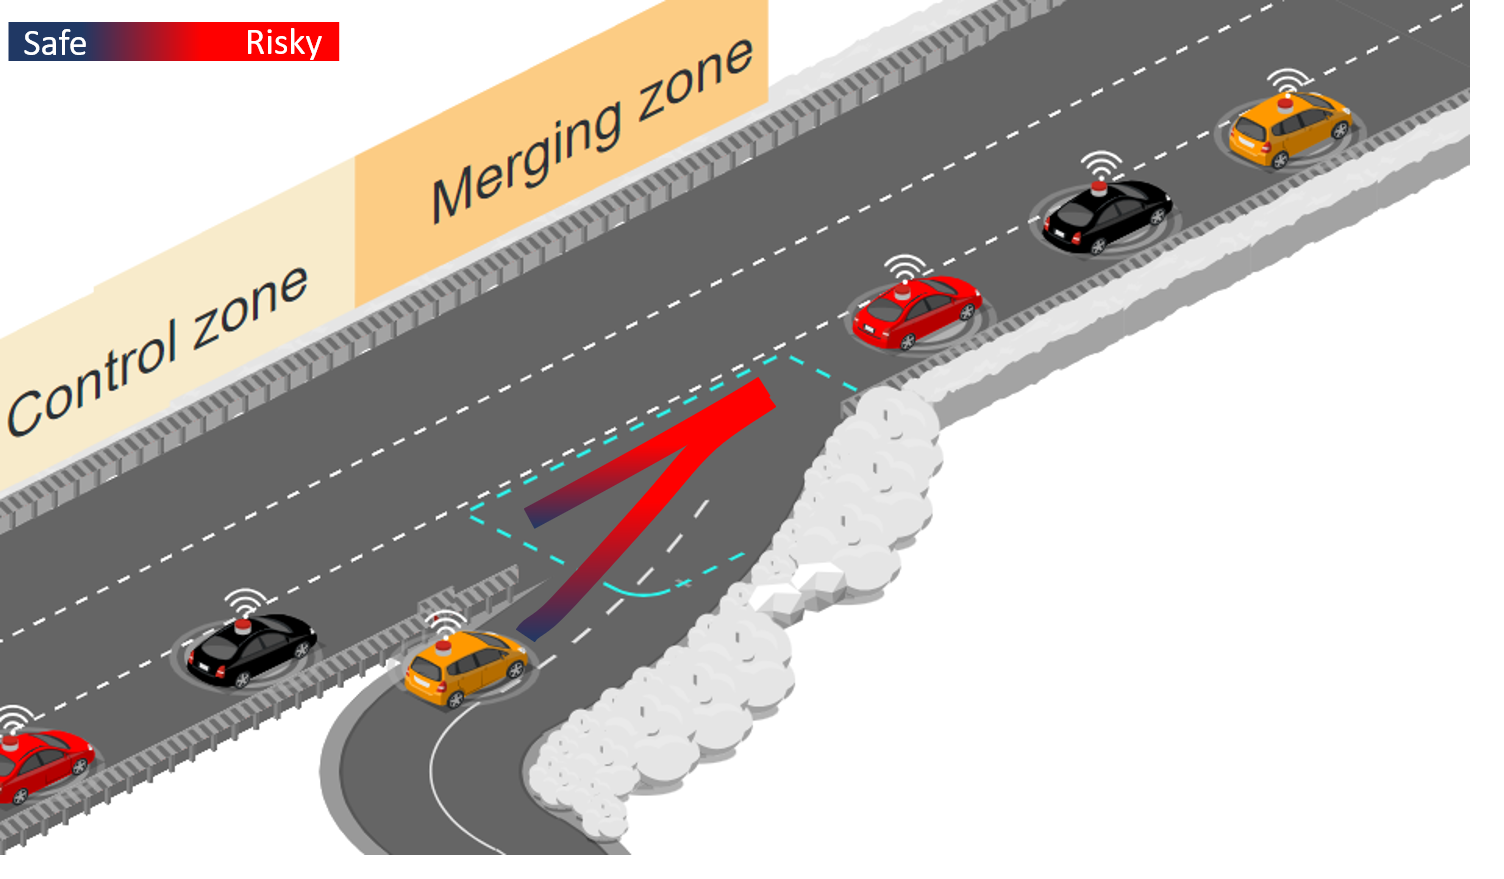
\includegraphics[width=10.5cm,height=18cm,keepaspectratio]{chapters/Chapitre_3/Figures/Cooperative_on_ramp_merging.png}
       % \vspace{-2.3mm}
        \caption{Decentralized collaborative on-ramp merging on highway}
        \label{fig:Decentralized_merging}
           %      \vspace{-5mm}
        \end{figure}}
In the virtual vehicle/platooning approach, each merging vehicle communicates its position and velocity within a certain range. Based on this data, each vehicle constructs its view of the merging scenario, replacing real-vehicles with virtual ones. Passing orders are then generated individually by each vehicle part of the MVS, aided by the virtualization. Conflict checks are performed to prevent merging collisions, with adjustments made if conflicts arise, depending on the merging strategy. An advanced variation of this approach introduced the concept of slots\footnote{ A slot is a geometrical space in the highway mainline, defined by its coordinates w.r.t. a common reference frame within the MVS, usually used by the vehicle for negotiation purposes to avoid collision}, allowing the vehicles part of the MVS to navigate within virtual slots. Conflict checking is conducted across these slots, accommodating localization uncertainties and ensuring minimal safety distances \cite{6338779}. In comparison with centralized methods, this cooperative merging method demonstrated superior performance in terms of traffic throughput and average on-ramp vehicle delay. %However, the level of conservativeness can vary based on slot dimensions, with slot-based virtual vehicle/platooning potentially being more conservative than the centralized approaches. 

\subsubsection{Energy efficiency} \label{sec: merging_energy_efficiency} 
Merging onto a dense highway from an on-ramp presents a complex challenge, characterized by its combinatorial nature and the limited information available regarding average speed in the different lanes \cite{7265166}. Additionally, ramp merging often leads to congestion and the formation of phantom traffic jams\footnote{Phantom traffic jams: dense traffic crawls to a halt for no apparent reason.} \cite{VAHIDI2018822}. V2V communication (cf. Section \ref{sec: communication}) offers a solution by enabling the anticipation of neighboring vehicles' intentions. This advanced knowledge of lane speeds can enhance the eco-driving control algorithms of MVS \cite{VAHIDI2018822}, resulting in more informed and smoother merging maneuvers. According to \cite{7313484} \cite{7562449}, these improvements can lead to an increased energy efficiency. Moreover, the benefits may extend beyond individual vehicles; by reducing the occurrence of phantom jams, the overall energy efficiency of traffic can be enhanced. However, it is worth noting that very few works have explored this particular advantage of MVS coordination on merging \cite{VAHIDI2018822}. %This scarcity of research can be attributed to the challenges associated with estimating fuel consumption, which is a complex task, and the intricate nature of on-ramp merging scenarios. Table \ref{energy} provides a summary of the limited findings regarding the impact of cooperative on-ramp merging on energy efficiency.


% \begin{table}[!ht]
% \renewcommand\arraystretch{1.25}
% \begin{adjustwidth}{-0.1\textwidth}{-0.1\textwidth}
% \caption{\label{energy}Summary of selected published results on energy efficiency gain enabled by anticipating margining on-ramp on highway.}
% \begin{tabularx}{\linewidth}{c c c } 
% \hline
% %\lipsum[11]\leavevmode\vspace*{-\baselineskip}
%  Reference &  Method and conditions & Energy efficiency (gain in \%)  \\ [0.8ex] 
%     \hline %%%%%%%%%%%%
%      \begin{minipage}{0.25\textwidth}   \vskip \cite{kamal2011ecological}  \vskip \end{minipage} &\Longstack{  \begin{minipage}{0.50\textwidth}   \vskip \begin{itemize} \setlength\itemsep{-0.4em} \item MPC velocity controller with $15\text{s}$ as prediction horizon  \end{itemize} \vskip  \end{minipage}} & \begin{minipage}{0.15\textwidth} \vskip  \empty{}\\\begin{itemize} \setlength\itemsep{-0.4em} \end{itemize} \vskip \end{minipage} \\  
%      \begin{minipage}{0.15\textwidth}   \vskip   \vskip \end{minipage} &\Longstack{  \begin{minipage}{0.50\textwidth}   \vskip \begin{itemize} \setlength\itemsep{-0.4em}  \item Simulation scenarios in $2\text{Km}$ road distance:  \subitem At $50\%$ MVS equipped with MPC controller w.r.t. conventional vehicles  \subitem At $50 \%$ MVS equipped with Cooperative Adaptive Cruise Control (CACC) w.r.t. conventional vehicles  \end{itemize} \vskip  \end{minipage}} & \begin{minipage}{0.15\textwidth} \vskip  \begin{itemize} \setlength\itemsep{-0.4em} \item $+12.9$ \\ \item $+7.5$  \end{itemize} \vskip \end{minipage} \\ 
%      \hline

%      %%%%%%%%
%      \begin{minipage}{0.25\textwidth}   \vskip \cite{7534837}  \vskip \end{minipage} &\Longstack{  \begin{minipage}{0.50\textwidth}   \vskip \begin{itemize} \setlength\itemsep{-0.4em} \item Optimal control based approach  \end{itemize} \vskip  \end{minipage}} & \begin{minipage}{0.15\textwidth} \vskip  \empty{}\\\begin{itemize} \setlength\itemsep{-0.4em} \end{itemize} \vskip \end{minipage} \\  
%      \begin{minipage}{0.15\textwidth}   \vskip   \vskip \end{minipage} &\Longstack{  \begin{minipage}{0.50\textwidth}   \vskip \begin{itemize} \setlength\itemsep{-0.4em}  \item Simulation scenarios:  \subitem  Coordination of $30 \text{vehicles}$ with same initial speed \subitem  Coordination of $30 \text{vehicles}$ With Different Initial Speed for Each Road \end{itemize} \vskip  \end{minipage}} & \begin{minipage}{0.15\textwidth} \vskip  \begin{itemize} \setlength\itemsep{-0.4em} \item $+52.7$ \\ \item $+48$  \end{itemize} \vskip \end{minipage} \\ 
%      \hline

%      %%%%%%%%
     
     
    
     
%     \hline

% \end{tabularx}
% \end{adjustwidth}
% \end{table}
% \\






\subsubsection{Negotiation} \label{sec: merging_negotiation}
In the absence of road coordinator and predefined heuristic rules, a vehicle seeking to merge into a lane from an on-ramp vehicle must ensure two conditions: (a) avoiding collisions with vehicles already in the targeted lane, and (b) executing a smooth merge without abruptly slowing down the vehicles on the target lane \cite{mariani2021coordination}. 

The approaches proposed in \cite{amoozadeh2015platoon} and \cite{aoki2017merging} rely on V2V communication (cf. Section \ref{sec: communication}) through the Vehicular Ad-Hoc network VANET protocol to facilitate negotiation. The merging vehicle initiates action proposals to vehicles already on the target lane, with the latter having the right to decline and propose alternative actions. In congested traffic conditions, such approaches are susceptible to issues of resource allocation, as vehicles on the highway may be unwilling or unable to accept proposals of cooperation from on-ramp vehicles. In other terms, the allocation of resources (space and time) for vehicles willing to merge from on-ramps to highway can be problematic due to reluctance or inability of vehicles already on the highway to accept this merging proposals. 

To address the challenge of resource allocation, negotiation approaches based on incentive mechanisms can be conceptualized. For instance, merging vehicles could employ auctions \cite{adhau2012multi}\cite{adnan2016protocols}\cite{cui2013game},where they offer compensation to enter the target lane. However, as of now, no relevant examples of such mechanisms have been found in the literature.


\section{Conclusion}


This chapter introduced various paradigms employed in the construction of the multi-vehicles system (MVS) control architecture. Additionally, it delved into the concept of formation control through a comprehensive review of the diverse approaches utilized for this purpose. Furthermore, this chapter explored the relevant literature concerning the versatile application of MVS, where the main challenges related to the different applications were highlighted. 

Addressing the challenges of MVS in dynamic and complex on-road environment, such as on-ramp merging and navigation in formation in highway, requires a multifaceted control architecture. The key takeaways from this chapter are listed as follows: 









\begin{enumerate}

    \item \textbf{Formal modeling of the MVS formation:} The formation composed by the vehicles part of the MVS should be done following a formal approach. Formal modeling helps to prove the stability of the formation motion, provides safety proofs, and enhances the cooperation efficiency. 

    \item \textbf{Distributed solution:} The proposed solution should aim for a high degree of decentralization to minimize dependencies on central units.

     \item \textbf{Promoting cooperation:} To prevent selfish behaviors, negotiation mechanisms should be an integral part of the solution to encourage cooperative interactions. Additionally, the notion of altruism coupled with MVS cooperation can be interesting to mitigate this issue. 

    
     \item \textbf{Performance demonstration:} The effectiveness of the proposed solution should be demonstrated in through the prism of its effects on safety, traffic flow, passenger comfort, and energy efficiency. 

    \item \textbf{Robustness:} The decision-making layer must prioritize robustness to ensure safe operations, and risk management methods should be integrated to maintain collision-free interactions.

     \item \textbf{Uncertainty assessment:} Recognizing that uncertainties are inherent to the problem, the proposed solution should incorporate mechanisms to address these uncertainties effectively.


\end{enumerate}

%% ajouter les deux références ci dessous à la partie navigation en formation dans le highway avec le concept de platoon virtuel 
% - W.J. Scholte, P.W.A. Zegelaar, H. Nijmeijer,
%A control strategy for merging a single vehicle into a platoon at highway on-ramps,Transportation Research Part C: Emerging Technologies, Volume 136,

% - Yongjie Xue, Xiaokai Zhang, Zhiyong Cui, Bin Yu, Kun Gao,
%A platoon-based cooperative optimal control for connected autonomous vehicles at highway on-ramps under heavy traffic, Transportation Research Part C: Emerging Technologies, 


























% l'idée de cette section est de donner des exmples d'application de la navigation en formaiton des MVS 
% \subsection{MVS navigation in formation: an application review}
% In the realm of MVS, the utilization of advanced formation methodologies has become pivotal in addressing a myriad of complex challenges mainly related to MVS' motion coordination. In particular, Cooperative Cruise Control (CACC) and consensus-base control strategies attention for their potential to improve the dynamics of MVS coordination. Building upon the fundamental concepts (cf. Section \ref{sec: formation_control_theory}), this section explores the multifaceted applications of CACC and consensus-based control within the realm of MVS. Through a comprehensive examination, it is proposed to delve into the intricacies of these control paradigms, shedding light to their promising contributions to enhancing on-road safety and transportation efficiency.







% Mes éléments c'est les suivants: 
% - navigation in formation  (application in highway - Leader follower, consensus based control) 
% - stategies used for on-ramp and off-ramp merging 
% - stategies used to MVS motion coordination - intersection crossing and roundbout 